% !TEX program = xelatex
% 中期答辩 PPT 大纲 —— 自动化实验部分 + 机器学习部分
% 编译：xelatex 两次
\documentclass[aspectratio=169,10pt]{ctexbeamer}

\usepackage{booktabs}
\usepackage{array}
\usepackage{tikz}
\usetikzlibrary{arrows.meta,positioning,shapes.geometric,calc,fit,backgrounds}
\usepackage{graphicx}
\usepackage{fontspec}
\setmainfont{Microsoft YaHei}
\setsansfont{Microsoft YaHei}

\usetheme{default}
\usecolortheme{default}
\setbeamertemplate{navigation symbols}{}
\setbeamertemplate{footline}[frame number]
\setbeamerfont{frametitle}{size=\large,series=\bfseries}
\setbeamercolor{frametitle}{fg=white,bg=blue!45!black}
\setbeamercolor{structure}{fg=blue!55!black}
\setbeamertemplate{itemize items}[circle]
\setbeamertemplate{blocks}[rounded][shadow=false]

% 图注命令：图 + 说明
\newcommand{\figslide}[3][0.86]{%
  \begin{center}\includegraphics[width=#1\textwidth,height=0.70\textheight,keepaspectratio]{img/#2}\end{center}%
  {\scriptsize\color{black!62}#3\par}%
}

\title{半挂车右转内轮差预警}
\subtitle{短时转角预测方法的仿真比较与性能代理模型}
\author{中期答辩}
\date{2026 年 10 月}

\begin{document}

% ======================================================================
\begin{frame}[plain]
  \titlepage
\end{frame}

\begin{frame}{本部分结构}
  \begin{columns}[T]
    \begin{column}{0.48\textwidth}
      \textbf{\color{blue!55!black}A. 自动化实验}
      \begin{enumerate}\small
        \item 研究问题与系统方案
        \item 实验组织：五层结构
        \item S1 核心方法对照
        \item S2 观测扰动
        \item S3 报警后处理
        \item S4 状态估计与增益精化
      \end{enumerate}
    \end{column}
    \begin{column}{0.48\textwidth}
      \textbf{\color{blue!55!black}B. 机器学习}
      \begin{enumerate}\small
        \item 为什么做代理模型
        \item 参数编码与输入向量
        \item 分组验证方案
        \item 五个模型族
        \item 结果：分档与外部检验
        \item 参数重要性
      \end{enumerate}
    \end{column}
  \end{columns}
  \vspace{0.6em}
  \begin{block}{一句话概括}
    \small 在固定的车辆几何与转弯条件下，用 39 条轨迹 × 70{,}000 个静态目标点，系统比较四种未来转角假设的预测精度与报警质量；再用代理模型检验这些规律能否被学出来并推广到新轨迹。
  \end{block}
\end{frame}

% ======================================================================
\section{A. 自动化实验}

\begin{frame}{A1\ \ 研究问题：内轮差为什么危险}
  \begin{columns}[T]
    \begin{column}{0.50\textwidth}
      \small
      \textbf{物理现象}\par
      半挂车右转时，挂车后轮走的弧线比牵引车更靠近弯心。
      行人往往在车头已经过去之后，才被向内切进来的挂车扫到。

      \vspace{0.7em}
      \textbf{本项目方案}\par
      ESP32 每 20\,ms 读取一次
      \begin{itemize}\small\setlength{\itemsep}{1pt}
        \item 车速 $v_B$
        \item 前轮转角 $\alpha$
        \item 铰接角 $\varphi$
      \end{itemize}
      用耦合运动学向前推\textbf{未来 2\,s 挂车右侧扫掠区}，
      目标落入即分级报警。

      \vspace{0.7em}
      \textbf{核心难题}\par
      未来 2\,s 内司机仍在打方向，$\alpha$ 在变。
      若假设 $\alpha$ 不变，入弯阶段会低估扫掠范围
      $\Rightarrow$ \textbf{报警偏晚}。
    \end{column}
    \begin{column}{0.48\textwidth}
      \begin{center}
      \begin{tikzpicture}[scale=0.84,>=Stealth,font=\scriptsize]
        % 危险带
        \fill[red!13] (0,3.4) arc (90:0:3.4) -- (5.4,0) arc (0:90:5.4) -- cycle;
        % 两条轨迹
        \draw[blue!60!black,line width=1.1pt] (0,5.4) arc (90:0:5.4);
        \draw[blue!60!black,line width=1.1pt,dashed] (0,3.4) arc (90:0:3.4);
        % 弯心
        \draw[black!55,line width=0.6pt] (-0.22,0)--(0.22,0);
        \draw[black!55,line width=0.6pt] (0,-0.22)--(0,0.22);
        \node[black!65,font=\tiny,below left] at (0,-0.10) {弯心 $O$};
        % 行驶方向
        \draw[->,black!55,line width=0.8pt] (0.42,4.35) arc (84:58:4.35);
        \node[black!60,font=\tiny] at (0.24,4.98) {行驶方向};
        % 内轮差标注
        \draw[<->,black!60,line width=0.6pt] (2.404,2.404)--(3.818,3.818);
        \node[black!75,font=\tiny,fill=white,inner sep=1pt,rotate=45] at (3.111,3.111) {内轮差};
        % 目标点
        \fill[red!80!black] (3.28,2.29) circle (2.3pt);
        \node[red!70!black,font=\tiny,right] at (3.44,2.22) {目标点};
      \end{tikzpicture}
      \end{center}
      {\scriptsize\color{black!70}%
      \tikz[baseline=-0.6ex]{\draw[blue!60!black,line width=1.1pt](0,0)--(0.55,0);}~牵引车右前轮轨迹\par
      \tikz[baseline=-0.6ex]{\draw[blue!60!black,line width=1.1pt,dashed](0,0)--(0.55,0);}~挂车右后轮轨迹（更靠弯心）\par
      \tikz[baseline=-0.6ex]{\fill[red!13](0,-0.07)rectangle(0.55,0.07);}~\textbf{红色带}：车头已过、车尾仍会扫到的区域\par}
    \end{column}
  \end{columns}
\end{frame}

\begin{frame}{A2\ \ 车辆模型与四种转角假设}
  \vspace{-0.15em}
  \begin{columns}[T]
    \begin{column}{0.45\textwidth}
      \small
      \textbf{耦合运动学}\quad{\footnotesize $l{=}4.0$, $l_h{=}1.8$, $L{=}13.5$, $W{=}2.0$\,m}
      \[
      \omega_1=\frac{v_B\tan\alpha}{l}
      \]
      \[
      \omega_2=\frac{v_B\sin\varphi+l_h\,\omega_1\cos\varphi}{L}
      \]
      \[
      \dot\varphi=\omega_1-\omega_2
      \]
      \vspace{0.15em}
      {\footnotesize $l_h\omega_1$ 为牵引销偏置耦合项，不可省略；RK4 积分，步长 0.02\,s。}

      \vspace{0.8em}
      \textbf{观测与限幅}\par
      \footnotesize
      用历史 0.2\,s 做因果二次拟合，得 $\dot\alpha,\ddot\alpha$；\newline
      $|\dot\alpha|\le32^\circ$/s，$|\ddot\alpha|\le160^\circ$/s$^2$，$|\alpha|\le30^\circ$。

      \vspace{0.8em}
      \textbf{三层扫掠区}\par
      \footnotesize
      同一套预测按未来时长切三层：W 2.0\,s（黄）、A 1.0\,s（红）、I 0.3\,s（紧迫）。
      每层用相邻步的右侧扫掠四边形拼接判定，保证时域单调。
    \end{column}
    \begin{column}{0.52\textwidth}
      \small
      \textbf{四种未来转角假设 $\alpha(u)$}\par
      \vspace{0.3em}
      {\scriptsize
      \renewcommand{\arraystretch}{1.32}
      \begin{tabular}{@{}l@{\hspace{7pt}}l@{}}
        \toprule
        方法 & 假设形式 \\
        \midrule
        保持 & $\alpha_0$ \\
        线性 & $\alpha_0+g\,\dot\alpha\,u$ \\
        衰减线性 & $\alpha_0+g\dot\alpha\tau'(1-e^{-u/\tau'})$ \\
         & \tiny$\tau'=\max(\tau,\ |g\dot\alpha|/160)$ \\
        受限二阶 & $\ddot\alpha$ 加速至多 $T_a$，之后保持 \\
        \bottomrule
      \end{tabular}}

      \vspace{1.0em}
      \textbf{\color{blue!55!black}同一帧、同样观测，2\,s 后 $\alpha$ 相差近 7 倍}\par
      \vspace{0.6em}
      \begin{center}
      \begin{tikzpicture}[x=0.29cm,y=0.72cm,>=Stealth,font=\tiny]
        \draw[->] (0,0)--(14.7,0);
        \draw[black!55] (0,0)--(0,3.55);
        \node[below,font=\tiny,align=center] at (9.2,-0.22) {$\alpha(2\,\mathrm{s})$ / $^\circ$};
        \fill[gray!55] (0,0.26) rectangle (2.0,0.60);
        \node[right,font=\tiny] at (2.10,0.43) {保持 2.0};
        \fill[blue!60!black] (0,1.16) rectangle (5.5,1.50);
        \node[right,font=\tiny] at (5.60,1.33) {衰减线性 5.5};
        \fill[cyan!65!black] (0,2.06) rectangle (6.0,2.40);
        \node[right,font=\tiny] at (6.10,2.23) {线性 6.0};
        \fill[red!70!black] (0,2.96) rectangle (13.8,3.30);
        \node[right,font=\tiny] at (13.87,3.13) {受限二阶 13.8};
      \end{tikzpicture}
      \end{center}
    \end{column}
  \end{columns}
\end{frame}

\begin{frame}{A3\ \ 实验怎么组织：五层结构}
  \vspace{-0.5em}
  \begin{center}
  \begin{tikzpicture}[scale=0.94,transform shape,node distance=0.26cm,>=Stealth,
      box/.style={draw,rounded corners=2pt,align=center,font=\scriptsize,
                  minimum height=1.02cm,text width=2.16cm,inner sep=1.5pt},
      lab/.style={font=\tiny\bfseries,text=white,inner sep=1.6pt,rounded corners=1pt}]

    % 五个阶段
    \node[box,fill=gray!10] (s0) {\textbf{S0}\\基础验收\\{\tiny 点密度/规模}};
    \node[box,fill=blue!10,right=of s0] (s1) {\textbf{S1}\\核心方法\\{\tiny 19 配置 × 27 轨迹}};
    \node[box,fill=blue!10,right=of s1] (s2) {\textbf{S2}\\观测扰动\\{\tiny 16 条件 × 3 预处理}};
    \node[box,fill=green!10,right=of s2] (s3) {\textbf{S3}\\后处理联合\\{\tiny 12 变体 × 39 轨迹}};
    \node[box,fill=orange!12,right=of s3] (s4) {\textbf{S4}\\状态估计\\{\tiny + 增益精化}};

    \draw[->,gray!65,line width=0.9pt] (s0)--(s1);
    \draw[->,gray!65,line width=0.9pt] (s1)--(s2);
    \draw[->,gray!65,line width=0.9pt] (s2)--(s3);
    \draw[->,gray!65,line width=0.9pt] (s3)--(s4);

    % 标签
    \node[lab,fill=gray!55,above=0.10cm of s0] {基础};
    \node[lab,fill=blue!55!black,above=0.10cm of s1] {方法};
    \node[lab,fill=blue!55!black,above=0.10cm of s2] {鲁棒性};
    \node[lab,fill=green!45!black,above=0.10cm of s3] {工程参数};
    \node[lab,fill=orange!65!black,above=0.10cm of s4] {补救};

    % 汇总条
    \node[draw,rounded corners=2pt,fill=gray!7,font=\scriptsize,align=center,
          below=0.60cm of s2,text width=12.4cm,inner sep=4pt] (agg) {
      \textbf{累计 3{,}585 个仿真作业}\quad
      S0 24 + S1 513 + S2 864 + S3 936 + S4a 576 + S4b 672\\
      {\tiny 作业 $=$ 1 条轨迹 $\times$ 1 个配置 $\times$ 1 种观测条件（S2 再乘 3 种输入处理，S0 为 12 条轨迹 $\times$ 2 种点密度）}
    };
  \end{tikzpicture}
  \end{center}

  \vspace{0.2em}
  \begin{block}{设计要点}
    \footnotesize
    \begin{itemize}\setlength{\itemsep}{2pt}
      \item \textbf{一次仿真} = 1 条轨迹 × 1 个配置 × 1 种观测条件；内部逐帧 1{,}854 次，每次判 70{,}000 个点。
      \item \textbf{每个阶段只改一个因子}，其余固定 $\Rightarrow$ 差异可归因到该因子。
      \item \textbf{预测结果可复用}：同一份预测序列套 12 种后处理参数 $\Rightarrow$ 作业数 $\ne$ 评分行数。
      \item 全部轨迹共享同一套目标坐标、接触标签、评分时段 $\Rightarrow$ 任意两配置可做逐轨迹配对差。
    \end{itemize}
  \end{block}
\end{frame}

\begin{frame}{A4\ \ 实验设计：因子与规模}
  \scriptsize
  \renewcommand{\arraystretch}{1.32}
  \begin{center}
  \begin{tabular}{@{}lccccccl@{}}
    \toprule
    \textbf{阶段} & \textbf{轨迹} & \textbf{配置} & \textbf{观测条件} & \textbf{后处理} & \textbf{输入处理} & \textbf{评分行} & \textbf{唯一自变量} \\
    \midrule
    S1 方法对照 & \textbf{27} & \textbf{19} & 1 & 1 & 1 & 513 & 算法配置（$g,\tau,T_a$）\\
    S2 观测扰动 & 6 & 3 & \textbf{16} & 1 & \textbf{3} & 864 & 噪声/延迟/预处理\\
    S3 后处理 & \textbf{39} & 3 & 8 & \textbf{12} & 1 & 7{,}800 & 窗口/膨胀/确认\\
    S4a 状态估计 & 6 & 3 & 8 & 1 & \textbf{4} & 576 & $\varphi$ EKF / $\alpha$ 低通\\
    S4b 增益精化 & \textbf{12}$^{*}$ & \textbf{7} & 8 & \textbf{12} & 1 & 8{,}064 & 增益联合调整\\
    \bottomrule
  \end{tabular}
  \end{center}
  {\tiny $^{*}$ S4b 使用 12 条\textbf{选择轨迹}（2.5/3.5\,m/s × 3/6\,°/s × 3 模板），与 27 条开发轨迹不重叠。}

  \vspace{0.5em}
  \begin{columns}[T]
    \begin{column}{0.47\textwidth}
      \textbf{27 条开发轨迹的因子设计}
      \begin{center}
      \begin{tabular}{@{}lc@{}}
        \toprule
        车速 $v_B$ & 2 / 3 / 4\,m/s \\
        基准转角速率 $r$ & 2 / 4 / 8\,°/s \\
        动作模板 & 对称 / 快入弯 / 快回正 \\
        转角峰值 & \textbf{10°（固定）}\\
        \bottomrule
      \end{tabular}
      \end{center}
    \end{column}
    \begin{column}{0.50\textwidth}
      \textbf{16 种观测条件}（S2）
      \begin{itemize}\tiny\setlength{\itemsep}{0pt}
        \item clean ×1
        \item 纯噪声 0.5/1/2 倍 × 3 种子 = 9
        \item 纯延迟 50/100/200\,ms = 3
        \item 噪声+延迟（1 倍 + 100\,ms）× 3 种子 = 3
      \end{itemize}
      \vspace{0.2em}
      {\tiny 噪声标准差（1 倍）：$\alpha$ 0.15°、$\varphi$ 0.25°、$v_B$ 0.04\,m/s}
    \end{column}
  \end{columns}
\end{frame}

\begin{frame}{A5\ \ 数据总览：轨迹与目标点}
  \vspace{-0.35em}
  \begin{columns}[T]
    \begin{column}{0.60\textwidth}
      \begin{center}
      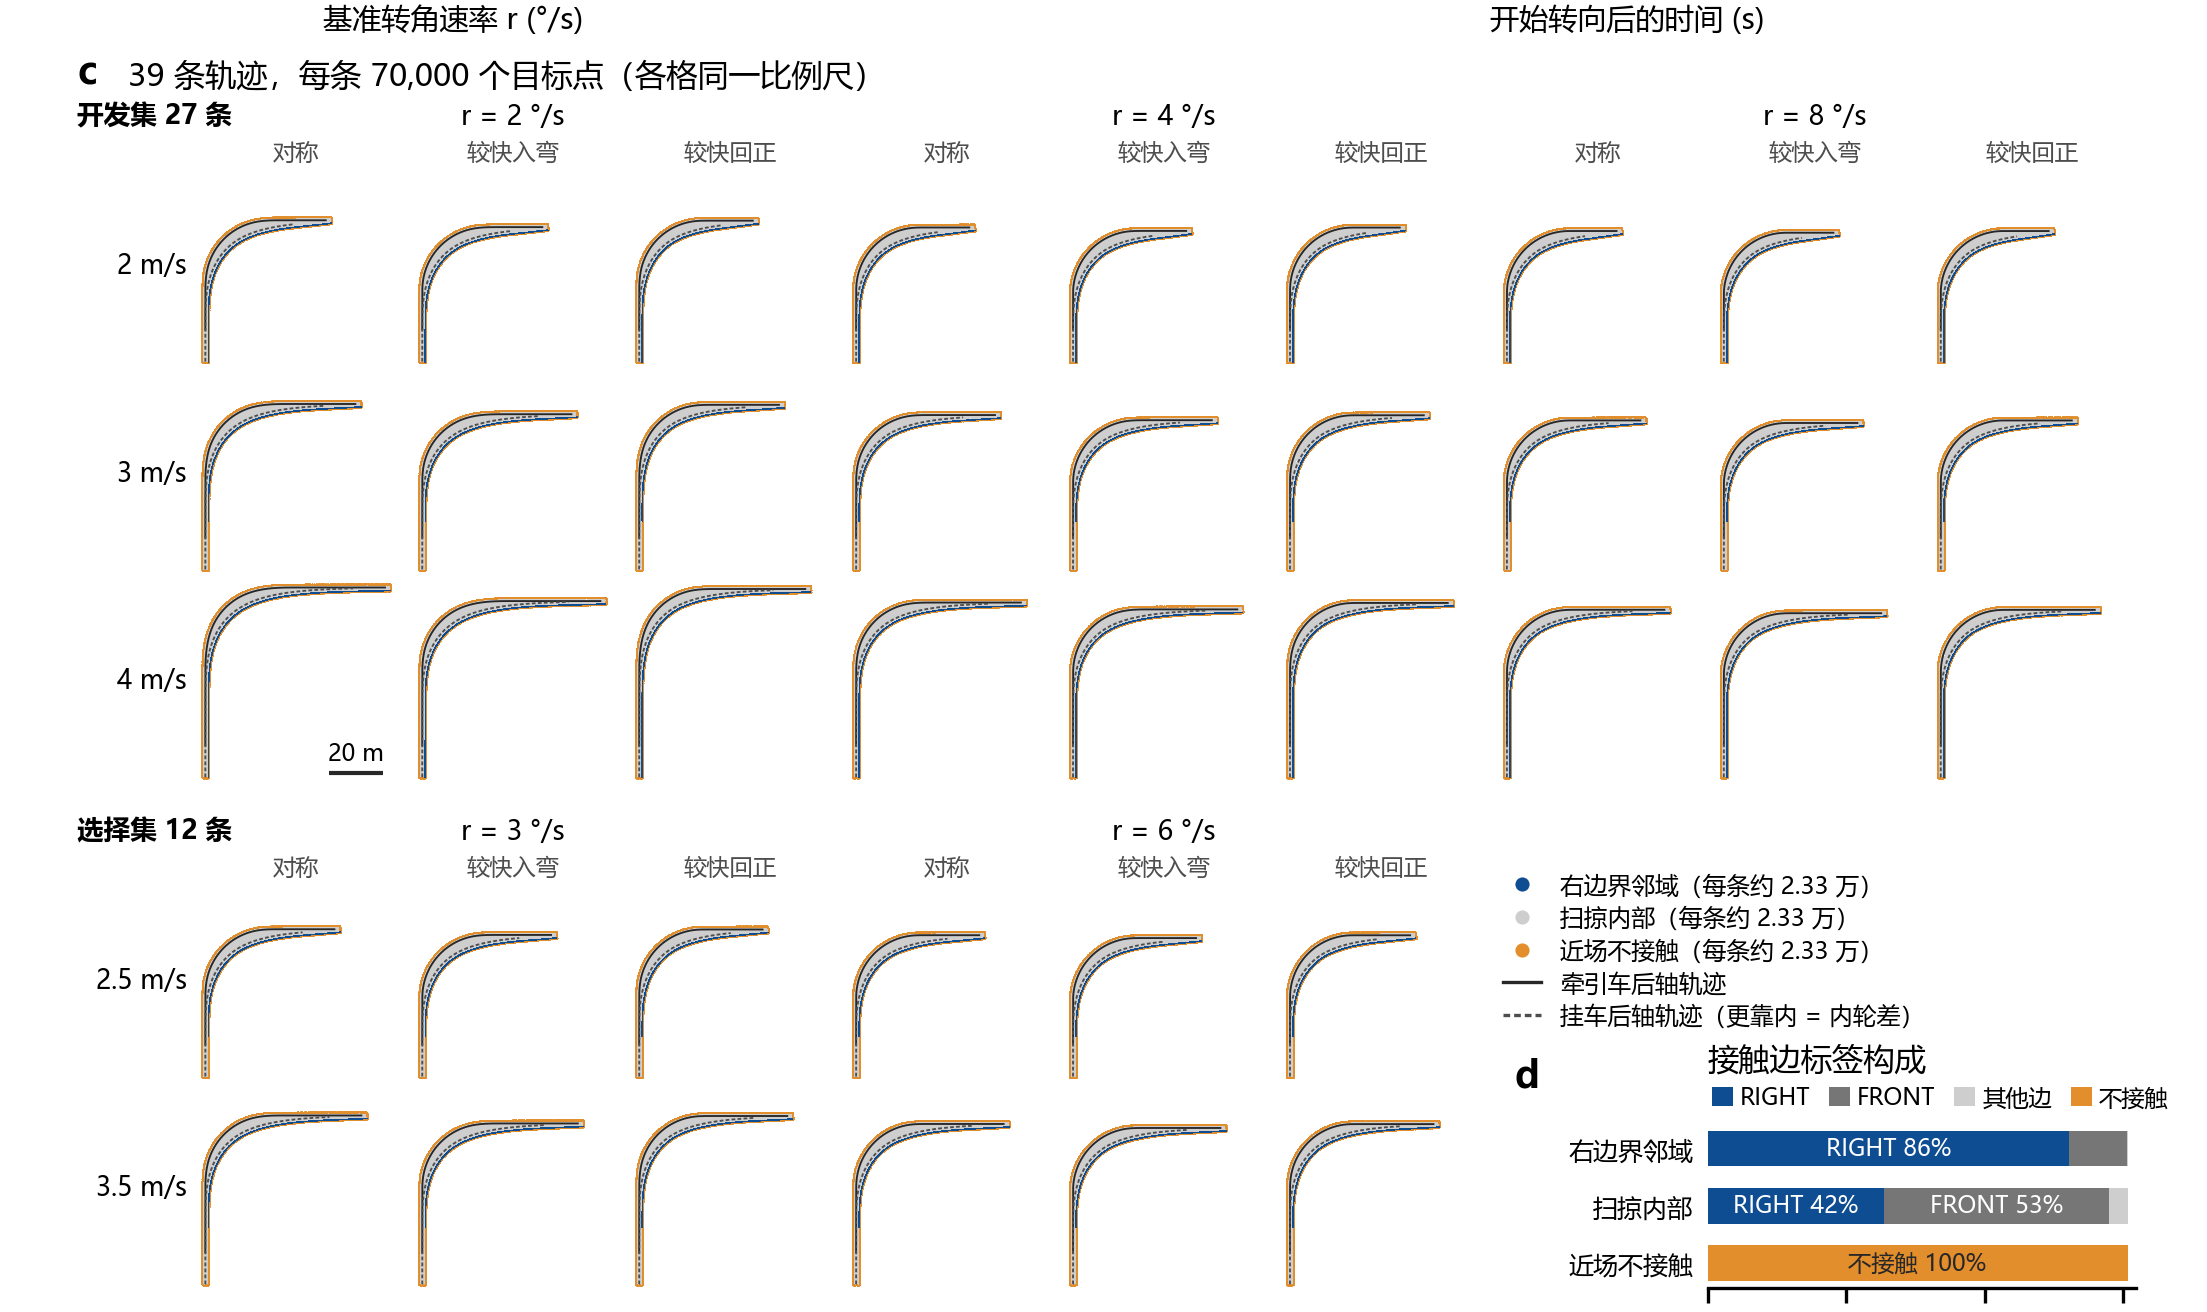
\includegraphics[width=\textwidth,height=0.70\textheight,keepaspectratio]{img/fig15_c.png}
      \end{center}
      {\scriptsize\color{black!62}39 条轨迹，同一比例尺；黑实线为牵引车后轴轨迹，灰虚线为挂车后轴轨迹（更靠内 $=$ 内轮差）。\par}
    \end{column}
    \begin{column}{0.38\textwidth}
      \footnotesize
      \textbf{每条轨迹 70{,}000 个静态目标点}\par
      按三个分层各约三分之一：
      \begin{enumerate}\footnotesize\setlength{\itemsep}{1pt}
        \item 右边界邻域（最终车身扫掠并集边界 0.20\,m 内且邻近右侧扫掠）
        \item 扫掠区内部
        \item 近场非接触（扫掠区外 0.05--0.50\,m）
      \end{enumerate}
      三等分等权，避免远处空地撑大负样本分母。

      \vspace{0.5em}
      \textbf{各层标签构成}\par
      \scriptsize
      右边界邻域：RIGHT 86\%；\\
      扫掠内部：RIGHT 42\%、FRONT 53\%；\\
      近场非接触：不接触 100\%。

      \vspace{0.7em}
      \begin{block}{关键}
        \scriptsize
        70{,}000 个点\textbf{不是} 70{,}000 次独立试验——最接近独立样本的单位是\textbf{轨迹}（27 或 39 条）。
      \end{block}
    \end{column}
  \end{columns}
\end{frame}

\begin{frame}{A6\ \ 案例：同一帧里三种方法的预测区}
  \vspace{-0.6em}
  \begin{center}
  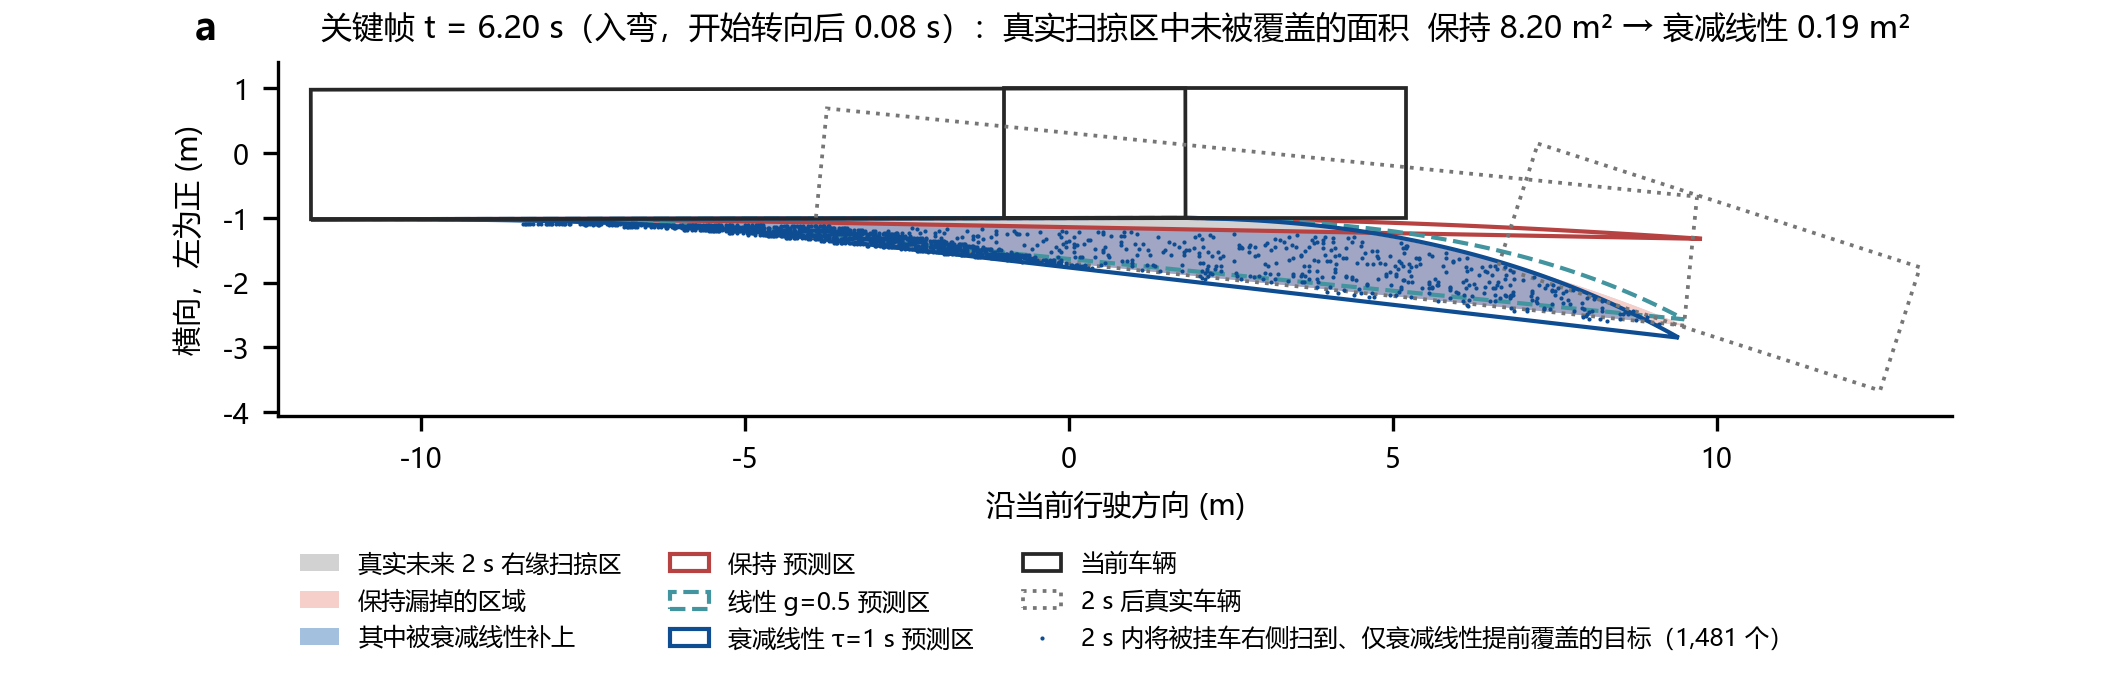
\includegraphics[width=0.985\textwidth,height=0.60\textheight,keepaspectratio]{img/fig13_panel_a.png}
  \end{center}
  \vspace{-0.35em}
  {\scriptsize\color{black!62}轨迹 \texttt{v4\_r8\_fast\_entry}（4\,m/s，入弯速率 16\,°/s），关键帧 $t$=6.20\,s（开始转向后 0.08\,s）。示意范围沿当前行驶方向。\par}
  \vspace{0.5em}
  {\footnotesize
  灰底 $=$ 真实未来 2\,s 右缘扫掠区；红框 $=$ 保持的预测区；蓝框 $=$ 衰减线性的预测区。
  \textbf{真实扫掠区中未被覆盖的面积}：保持 \textbf{8.20\,m$^2$} $\rightarrow$ 衰减线性 \textbf{0.19\,m$^2$}，
  补上 8.00\,m$^2$，涉及 \textbf{1{,}481} 个目标点。
  这是差别最大的一帧，用来说明机制，\textbf{不代表一般改善幅度}。}
\end{frame}

\begin{frame}{A7\ \ 案例：报警—接触时间轴}
  \vspace{-0.5em}
  \begin{columns}[T]
    \begin{column}{0.46\textwidth}
      \begin{center}
      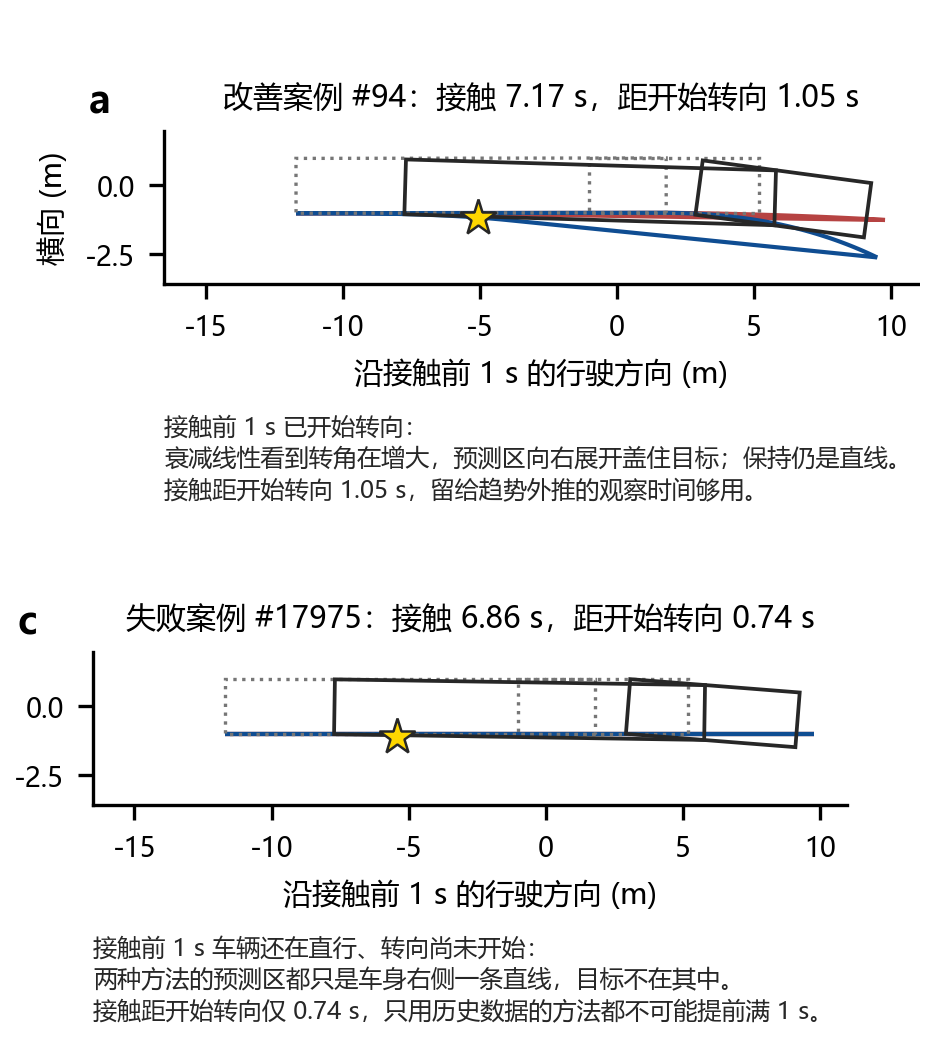
\includegraphics[width=\textwidth,height=0.735\textheight,keepaspectratio]{img/fig14_cases.png}
      \end{center}
    \end{column}
    \begin{column}{0.51\textwidth}
      \footnotesize
      \textbf{红色 $=$ 保持的预测区（接触前 1\,s）；蓝色 $=$ 衰减线性的预测区；黄星 $=$ 目标点}\par

      \vspace{0.9em}
      \textbf{改善案例 \#94}\par
      接触前 1\,s 已开始转向：衰减线性看到转角在增大，预测区向右展开盖住目标；保持仍是直线，盖不住。
      接触距开始转向 1.05\,s，\textbf{留给趋势外推的时间够用}。

      \vspace{0.9em}
      \textbf{失败案例 \#17975}\par
      接触前 1\,s 车辆还在直行、转向尚未开始：两种方法的预测区都只是车身右侧一条直线。
      接触距开始转向仅 0.74\,s，\textbf{只用历史数据的方法都不可能提前 1\,s}。

      \vspace{1.0em}
      \textbf{全轨迹统计}\par
      20{,}369 个 RIGHT 接触目标中，提前量不足 1\,s 的从保持 \textbf{852} 个降到衰减线性 \textbf{512} 个
      （改善 340 个，\textbf{无一个变差}）。仍迟报的 512 个里 \textbf{96\%} 在开始转向后 1\,s 内接触。
    \end{column}
  \end{columns}
\end{frame}

\begin{frame}{A8\ \ S1 结果：2\,s 端点误差最小的是适度外推}
  \vspace{-0.35em}
  \begin{center}
  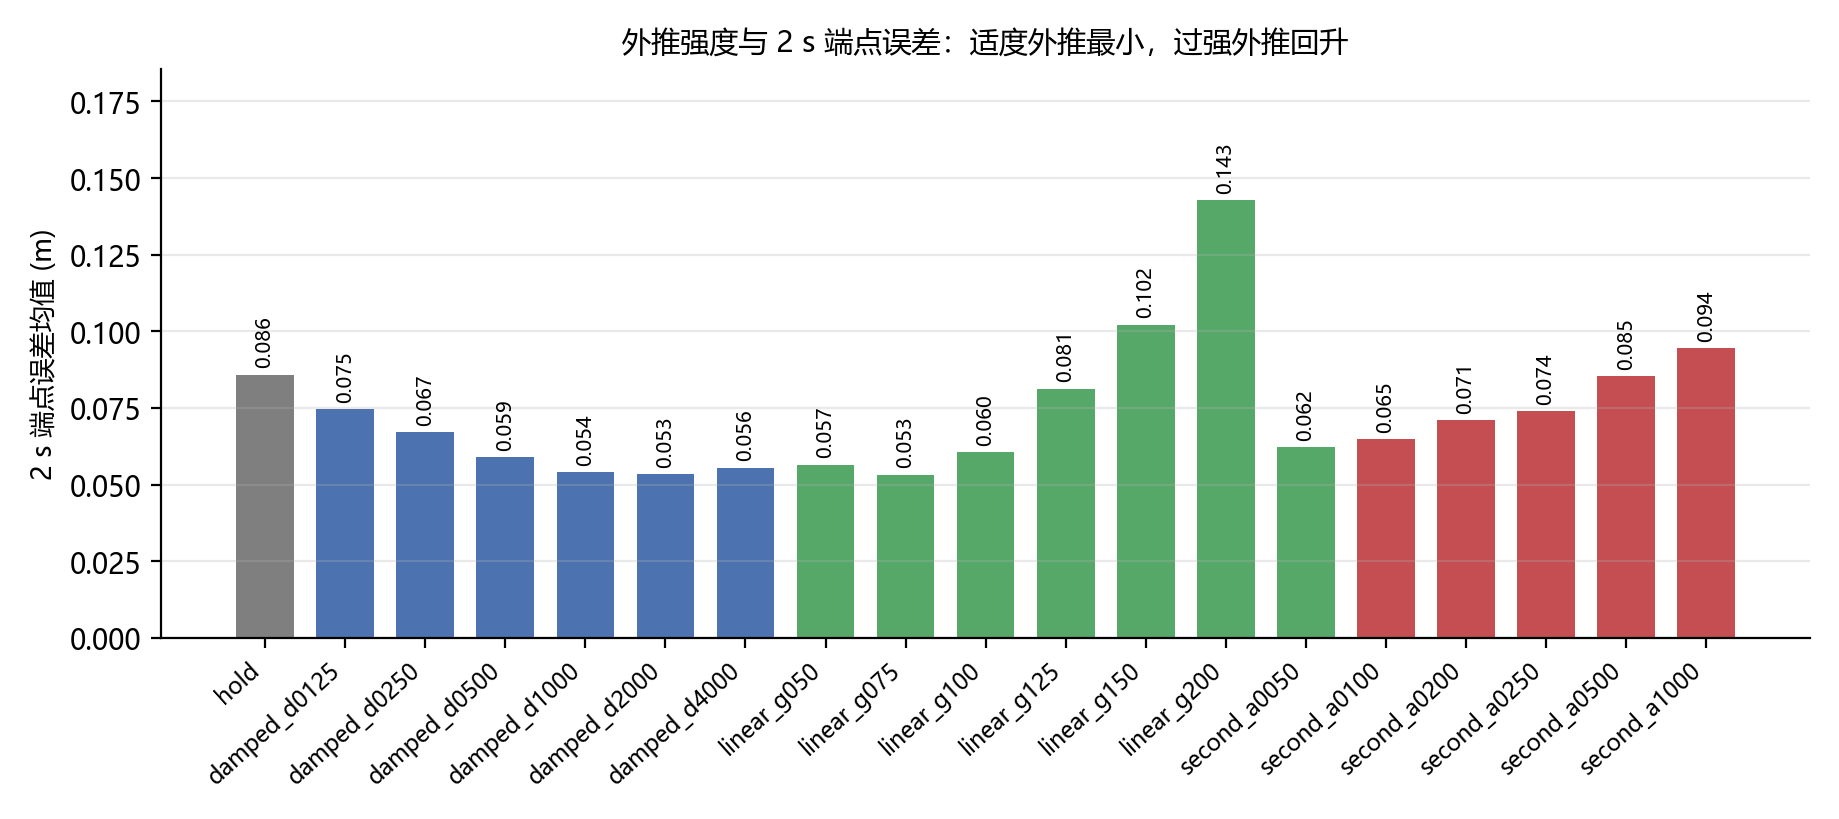
\includegraphics[width=0.94\textwidth,height=0.615\textheight,keepaspectratio]{img/a8_geom_bar.png}
  \end{center}
  \vspace{-0.5em}
  {\footnotesize
  \textbf{端点误差是纯几何量}（预测 2\,s 后右缘端点 vs 真实端点），\textbf{不依赖接触标签}。
  保持 \textbf{0.086\,m}$\rightarrow$\texttt{linear\_g075} \textbf{0.053\,m}、\texttt{damped\_d2000} 0.053\,m（\textbf{降 38\%}）；
  外推过强反而回升：\texttt{linear\_g200} \textbf{0.143\,m}（比保持大 66\%），受限二阶 \texttt{second\_a1000} 也到 0.094\,m。
  \textbf{结论}：趋势外推必须\textbf{有界}。}
\end{frame}

\begin{frame}{A9\ \ S1 结果：配对迟报差（核心结论）}
  \vspace{-0.35em}
  \begin{center}
  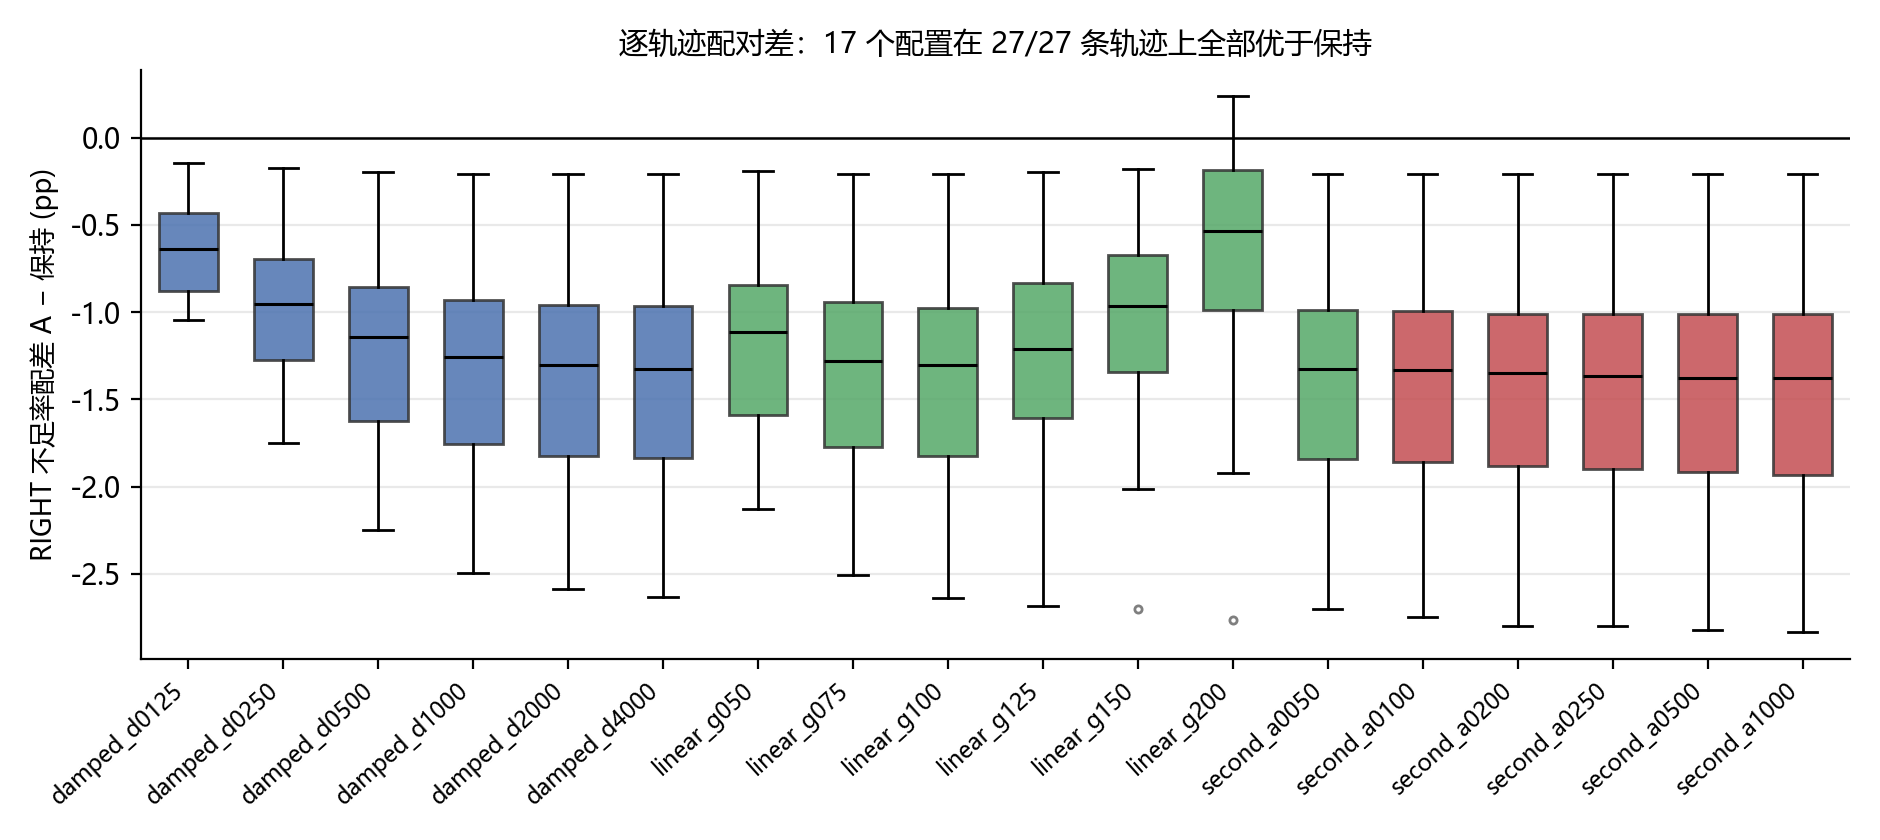
\includegraphics[width=0.96\textwidth,height=0.60\textheight,keepaspectratio]{img/a9_paired_late.png}
  \end{center}
  \vspace{-0.5em}
  {\footnotesize
  \textbf{同一条轨迹上}该配置的 RIGHT 不足率减去保持的，单位 pp；箱体是 27 条轨迹的四分位范围。
  \textbf{17 个配置在 27/27 条轨迹上全部优于保持}，唯一例外是外推最强的 \texttt{linear\_g200}（23/27）。
  平均降低 \textbf{0.66--1.47\,pp}。\textbf{这是本阶段最强的一条结论}：不是平均效应，而是\textbf{逐条成立}。}
\end{frame}

\begin{frame}{A10\ \ S1 结果：迟报与误报的权衡}
  \vspace{-0.35em}
  \begin{center}
  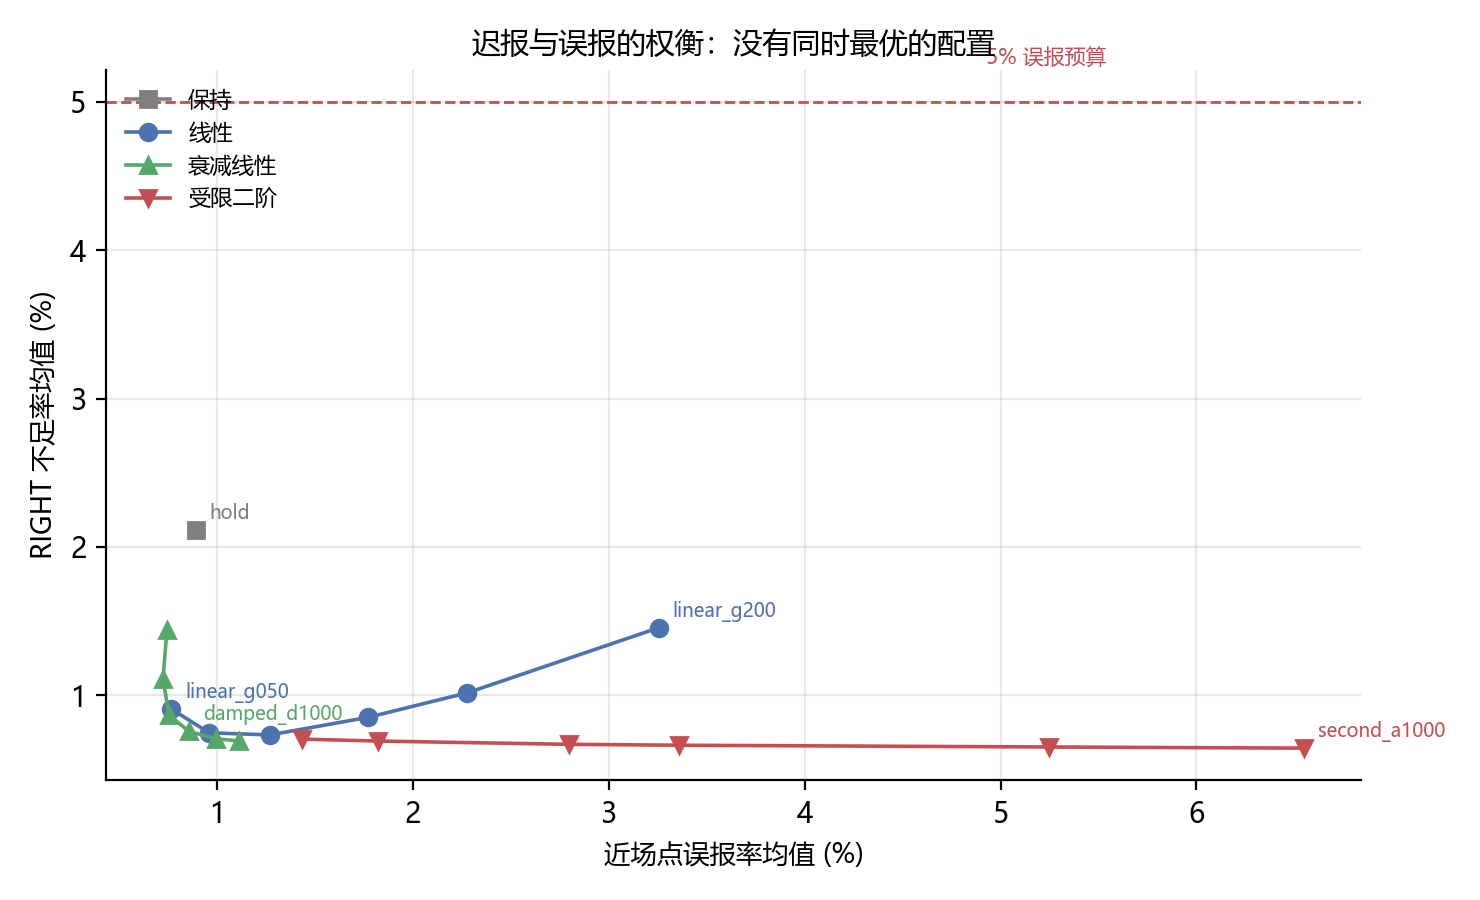
\includegraphics[width=0.80\textwidth,height=0.615\textheight,keepaspectratio]{img/a10_tradeoff.png}
  \end{center}
  \vspace{-0.45em}
  {\footnotesize
  从保持到 \texttt{damped\_d1000}：迟报 \textbf{2.11\%}$\rightarrow$\textbf{0.76\%}（降 64\%），
  误报 0.89\%$\rightarrow$0.86\%（\textbf{几乎不变}）——真正的双赢。
  但外推配置\textbf{之间}严格此消彼长：迟报最低的 \texttt{second\_a1000}（0.64\%）误报升到 \textbf{6.55\%}，超 5\% 预算。
  \textbf{所以后续只保留} \texttt{linear\_g050} 与 \texttt{damped\_d1000} 两个折点附近的方案。}
\end{frame}

\begin{frame}{A11\ \ 收益随车速与转向速率增大}
  \vspace{-0.35em}
  \begin{center}
  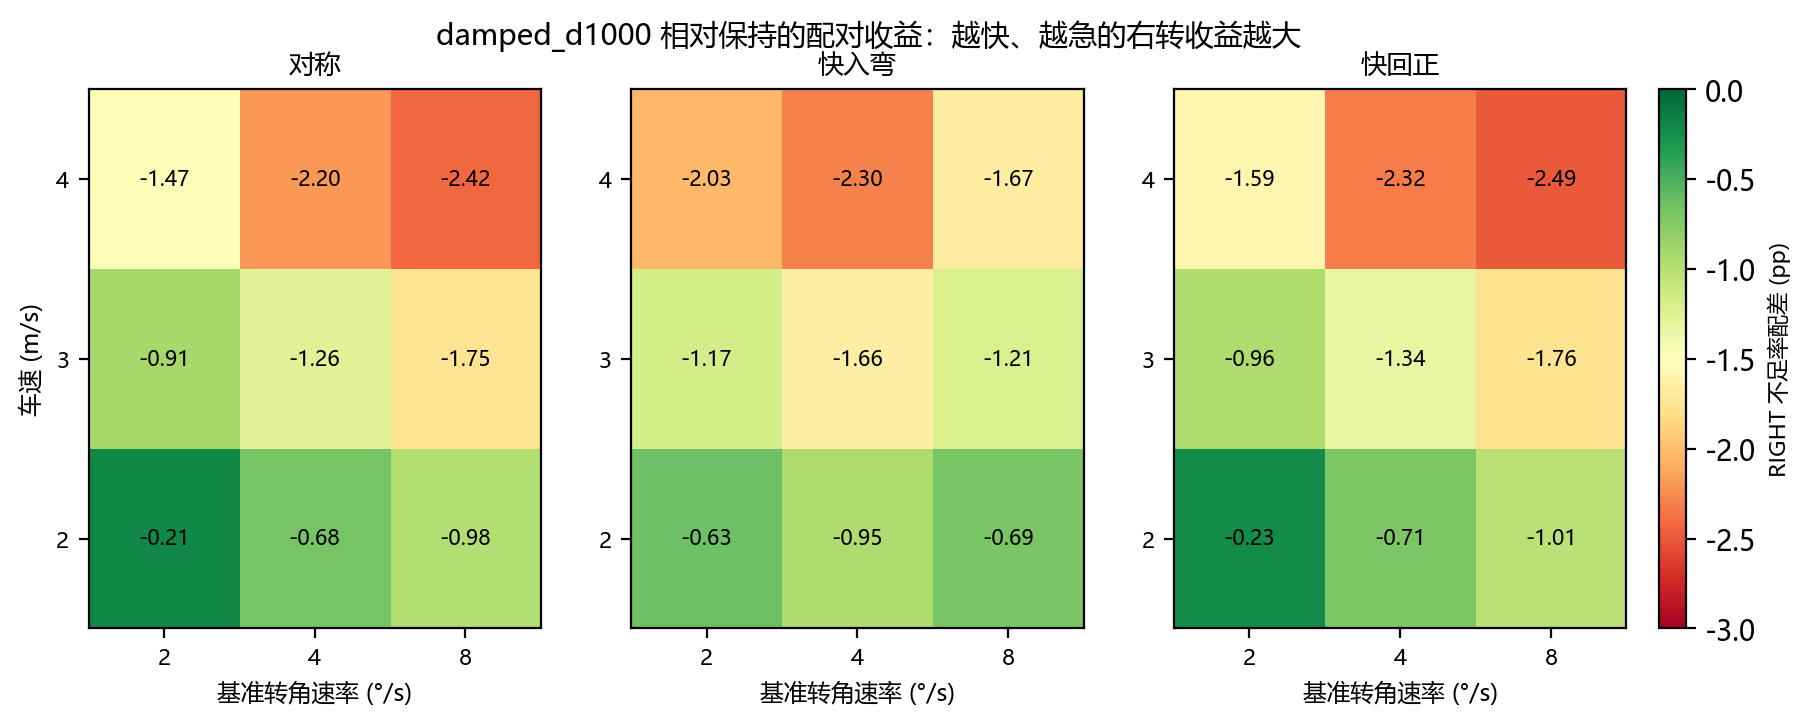
\includegraphics[width=0.97\textwidth,height=0.635\textheight,keepaspectratio]{img/a11_factor_heatmap.png}
  \end{center}
  \vspace{-0.45em}
  {\footnotesize
  以 \texttt{damped\_d1000} 为例（其余 17 个配置方向一致）：\textbf{27 格全部为负}。
  收益最小 \textbf{$-$0.21\,pp}（2\,m/s、2\,°/s、对称），最大 \textbf{$-$2.49\,pp}（4\,m/s、8\,°/s、快回正）。
  \textbf{越快、越急的右转，越需要预测转角趋势}。每格仅 1 条轨迹，看整体趋势而非单格数值。}
\end{frame}

\begin{frame}{A12\ \ S2：噪声主要抬误报，延迟主要抬迟报}
  \vspace{-0.4em}
  \begin{center}
  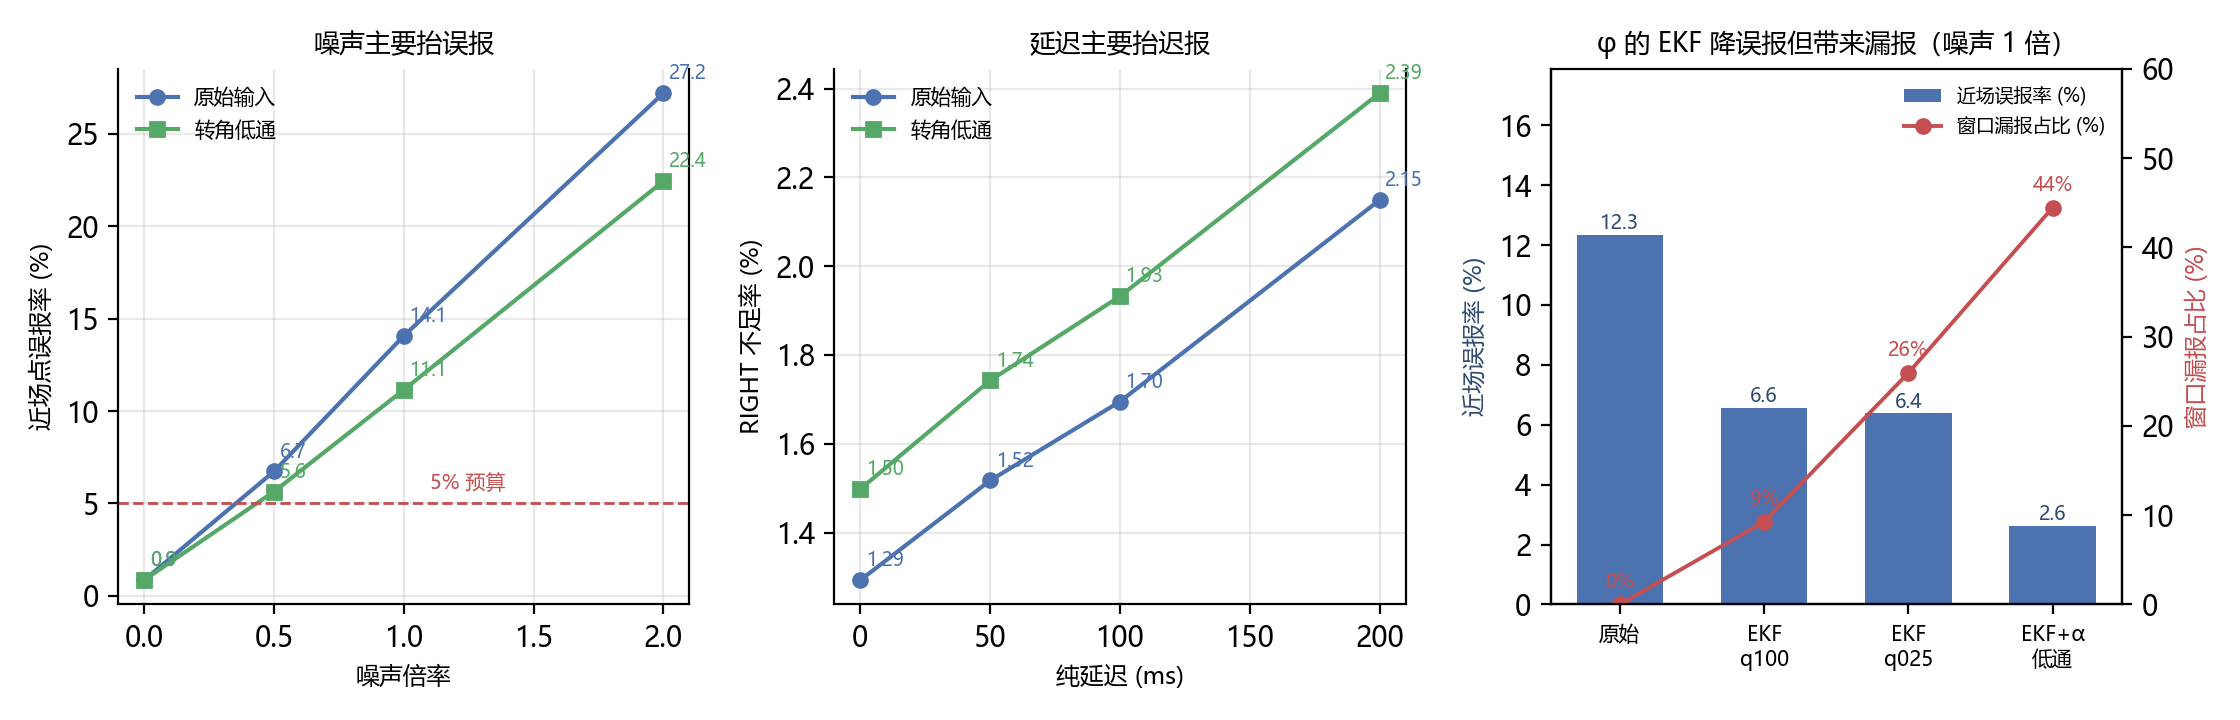
\includegraphics[width=0.985\textwidth,height=0.555\textheight,keepaspectratio]{img/a12_noise_delay.png}
  \end{center}
  \vspace{-0.35em}
  {\footnotesize
  \textbf{左}（3 个种子平均）：原始输入下近场误报率 \textbf{0.85\%}$\rightarrow$\textbf{6.7\%}$\rightarrow$\textbf{14.1\%}$\rightarrow$\textbf{27.2\%}（噪声 0/0.5/1/2 倍），
  \textbf{0.5 倍噪声即超 5\% 预算}；转角低通把它降到 5.6/11.1/22.4\%。
  \textbf{中}：迟报率随延迟 \textbf{1.29\%}$\rightarrow$\textbf{2.15\%}（0$\rightarrow$200\,ms），点级误报几乎不变。
  \textbf{右}（噪声 1 倍）：$\varphi$ 的 EKF 把误报从 12.3\% 降到 6.6\%（q100）/6.4\%（q025）/2.6\%（+$\alpha$ 低通），
  但\textbf{窗口漏报占比从 0\% 升到 9\%/26\%/44\%}。}
\end{frame}

\begin{frame}{A13\ \ S3：后处理是最强旋钮，但各有代价}
  \vspace{-0.55em}
  \begin{columns}[T]
    \begin{column}{0.50\textwidth}
      \begin{center}
      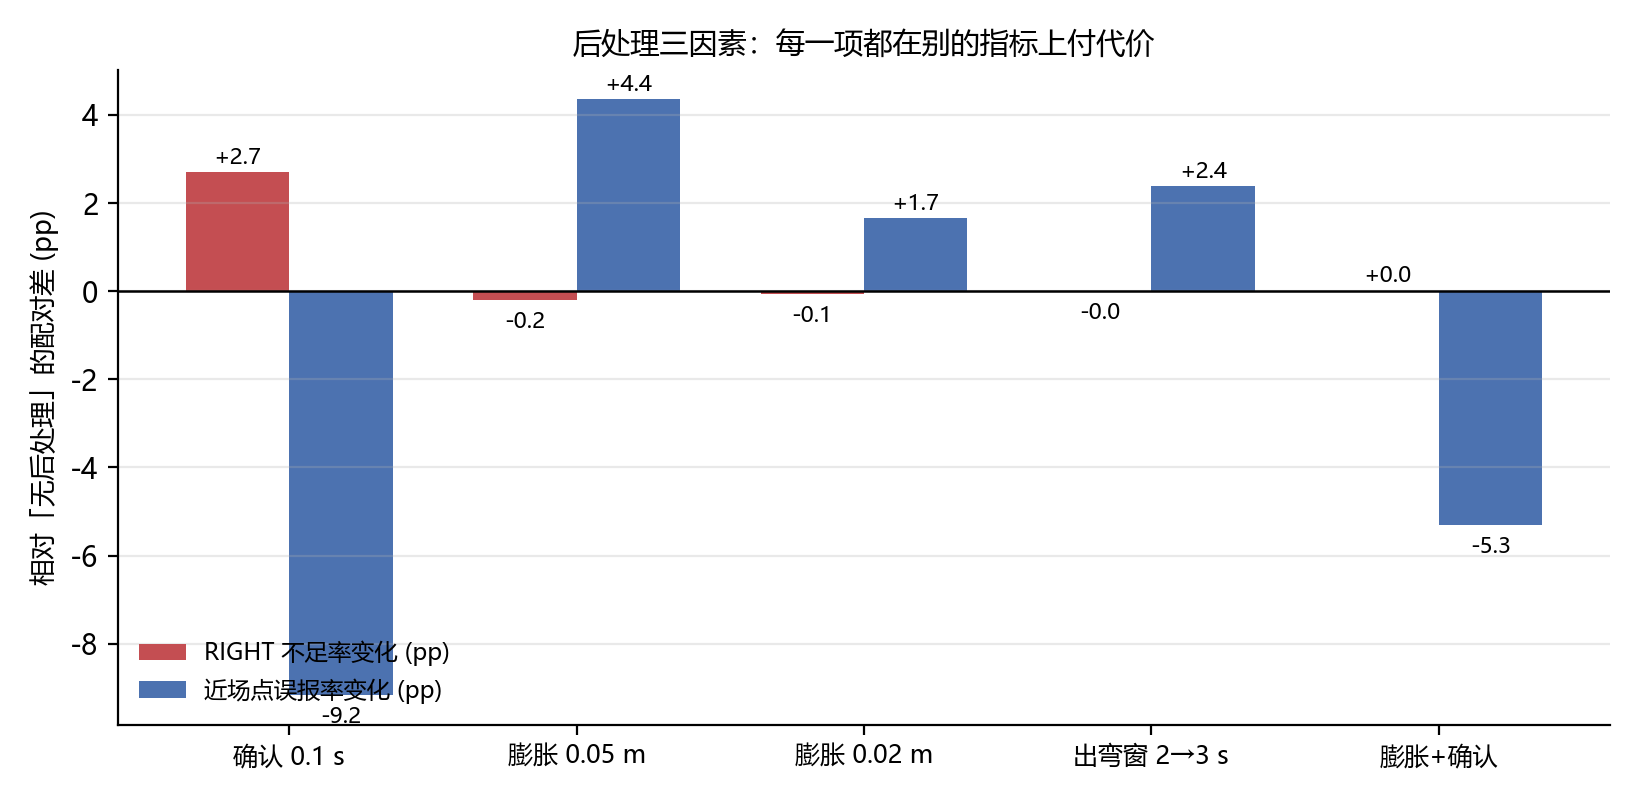
\includegraphics[width=\textwidth,height=0.70\textheight,keepaspectratio]{img/a13_postproc.png}
      \end{center}
    \end{column}
    \begin{column}{0.47\textwidth}
      \scriptsize
      \renewcommand{\arraystretch}{1.26}
      \begin{tabular}{@{}lrrr@{}}
        \toprule
        变体 & $\Delta$RIGHT & $\Delta$误报 & 窗口漏报 \\
        \midrule
        确认 0.1\,s & $+2.70$ & $-9.16$ & $+75$\% \\
        膨胀 0.05\,m & $-0.21$ & $+4.35$ & 0 \\
        膨胀 0.02\,m & $-0.06$ & $+1.66$ & 0 \\
        出弯窗 2→3\,s & $0.00$ & $+2.38$ & 0 \\
        膨胀+确认 & $+0.01$ & $-5.32$ & 0 \\
        \bottomrule
      \end{tabular}
      \vspace{0.35em}

      {\tiny\color{black!62}$\Delta$ 为相对「无后处理」的 624 组逐轨迹配对差均值（pp）。}

      \vspace{0.8em}
      \footnotesize
      \textbf{确认 0.1\,s} 把误报砍掉 9\,pp，但 RIGHT 不足率 +2.7\,pp，且 \textbf{75\% 的作业出现窗口漏报}——
      压掉的是真实的早期报警。

      \vspace{0.6em}
      \textbf{膨胀 0.05\,m} 方向相反：误报 +4.4\,pp，迟报只降 0.2\,pp，性价比最低。

      \vspace{0.6em}
      \textbf{出弯窗口 2→3\,s}：$\Delta$RIGHT 恰为 0，\textbf{只增加误报}。
      膨胀+确认合用能回到 $-5.3$\,pp 误报而不伤迟报，是唯一可接受的组合。
    \end{column}
  \end{columns}
\end{frame}

\begin{frame}{A14\ \ S4 联合精化：增益不必细调}
  \vspace{-0.4em}
  \begin{columns}[T]
    \begin{column}{0.52\textwidth}
      \footnotesize
      \renewcommand{\arraystretch}{1.30}
      \begin{tabular}{@{}lcc@{}}
        \toprule
        \textbf{方法 / 增益} & \textbf{RIGHT 不足率} & \textbf{近场误报率} \\
        \midrule
        保持 & 1.10\% & 7.28\% \\
        \midrule
        线性 $g$=0.375 & 0.34\% & 8.09\% \\
        线性 $g$=0.500 & 0.28\% & 9.00\% \\
        线性 $g$=0.625 & 0.24\% & 10.13\% \\
        \midrule
        衰减线性 $g$=0.75 & 0.28\% & 8.73\% \\
        衰减线性 $g$=1.00 & 0.23\% & 10.09\% \\
        衰减线性 $g$=1.25 & 0.21\% & 11.74\% \\
        \bottomrule
      \end{tabular}

      \vspace{0.8em}
      {\scriptsize\color{black!62}12 条选择轨迹、clean 条件、\textbf{无后处理}；数值为该组均值。}

      \vspace{1.0em}
      {\scriptsize\color{black!70}%
      \textbf{读表}：从保持切到任意外推，迟报一次掉 0.8\,pp 以上；
      之后每升一档增益，迟报最多再降 0.07\,pp，误报却涨 0.9--1.7\,pp。}
    \end{column}
    \begin{column}{0.45\textwidth}
      \footnotesize
      \textbf{好消息：增益不必细调}\par
      从保持切到任一趋势外推，RIGHT 不足率从 \textbf{1.10\%} 掉到 \textbf{0.21--0.34\%}，
      降幅的\textbf{绝大部分}在第一步就拿到了。

      \vspace{1.0em}
      \textbf{坏消息：再调是负和}\par
      在折点附近每升一档，迟报只再降 \textbf{0.03--0.07\,pp}，
      但近场误报升 \textbf{0.9--1.7\,pp}——\textbf{代价远大于收益}。

      \vspace{1.0em}
      \textbf{结论}\par
      继续优化的重点在\textbf{后处理与观测质量}，不在增益。
      这也解释了为什么 S3 的后处理效应（可达 $\pm$9\,pp）远大于增益精化（$\pm$0.07\,pp）。
    \end{column}
  \end{columns}
\end{frame}

\begin{frame}{A15\ \ 标签不确定性下的配对差区间}
  \figslide[0.76]{fig12_label_interval.png}{%
  对每个目标的接触时间在其允许区间内取极值，求配对差的上下界。
  clean（$\tau$=1\,s）：\textbf{$-$0.236 \dots $-$0.233\,pp}，区间宽仅 \textbf{0.003\,pp}；
  delay100：$-$0.587 \dots $-$0.571\,pp，\textbf{全在 0 以下}。
  噪声条件下区间跨 0 或恰为 0 $\Rightarrow$ \textbf{噪声会淹没方法间差异}，方向不能确定。
  注意：仅 1 条轨迹（车速最低、转向最慢，属保守旁证）。}
\end{frame}

% ======================================================================
\section{B. 机器学习}

\begin{frame}{B1\ \ 为什么做代理模型}
  \small
  每个评分行都是「一组实验设置 $\rightarrow$ 一组评分」。
  代理模型用\textbf{设置}预测\textbf{评分}，有三个用途：

  \vspace{0.4em}
  \begin{enumerate}\setlength{\itemsep}{2pt}
    \item \textbf{检验规律是否稳定}：连没见过的轨迹都能预测准 $\Rightarrow$ 评分随设置的变化有规律，不是噪声
    \item \textbf{量化各因素的作用}：置换重要性给出排序，部分依赖给出方向
    \item \textbf{为后续实验挑选值得仿真的设置}（减少盲目遍历）
  \end{enumerate}

  \vspace{0.7em}
  \begin{center}
  \begin{tikzpicture}[node distance=0.5cm,>=Stealth,
      b/.style={draw,rounded corners=2pt,align=center,font=\scriptsize,
                minimum height=1.62cm,text width=3.60cm,inner sep=3pt}]
    \node[b,fill=blue!8] (x) {\textbf{输入：实验设置}\\[2pt]
      {\tiny 工况：车速、入弯/回正速率、动作模板\\
       观测：噪声倍率、延迟、状态估计\\
       算法：方法、$g$、$\tau$、$T_a$、后处理}};
    \node[b,fill=gray!10,right=1.05cm of x] (f) {\textbf{代理模型}\\[2pt]
      {\tiny 梯度提升 / Ridge / 随机森林\\[2pt]
       \textbf{按轨迹分组}的交叉验证}};
    \node[b,fill=red!8,right=1.05cm of f] (y) {\textbf{输出：评分}\\[2pt]
      {\tiny RIGHT 不足率、误报率\\
       窗口漏报率、提前量 P10\\
       2\,s 端点误差}};
    \draw[->,gray!70,line width=1pt] (x)--(f);
    \draw[->,gray!70,line width=1pt] (f)--(y);
  \end{tikzpicture}
  \end{center}

  \vspace{0.6em}
  \begin{alertblock}{边界}
    \footnotesize
    代理模型是\textbf{电脑端分析工具}，不进车载预测器，也不作为安全结论。
    输入端只用\textbf{工况 + 观测条件 + 生效算法参数}；
    未来动作、真值接触时间、作业 ID、已有评分\textbf{一律不作输入}。
  \end{alertblock}
\end{frame}

\begin{frame}{B2\ \ 参数编码：11 个数值 + 2 个类别}
  \vspace{-0.4em}
  \begin{center}
    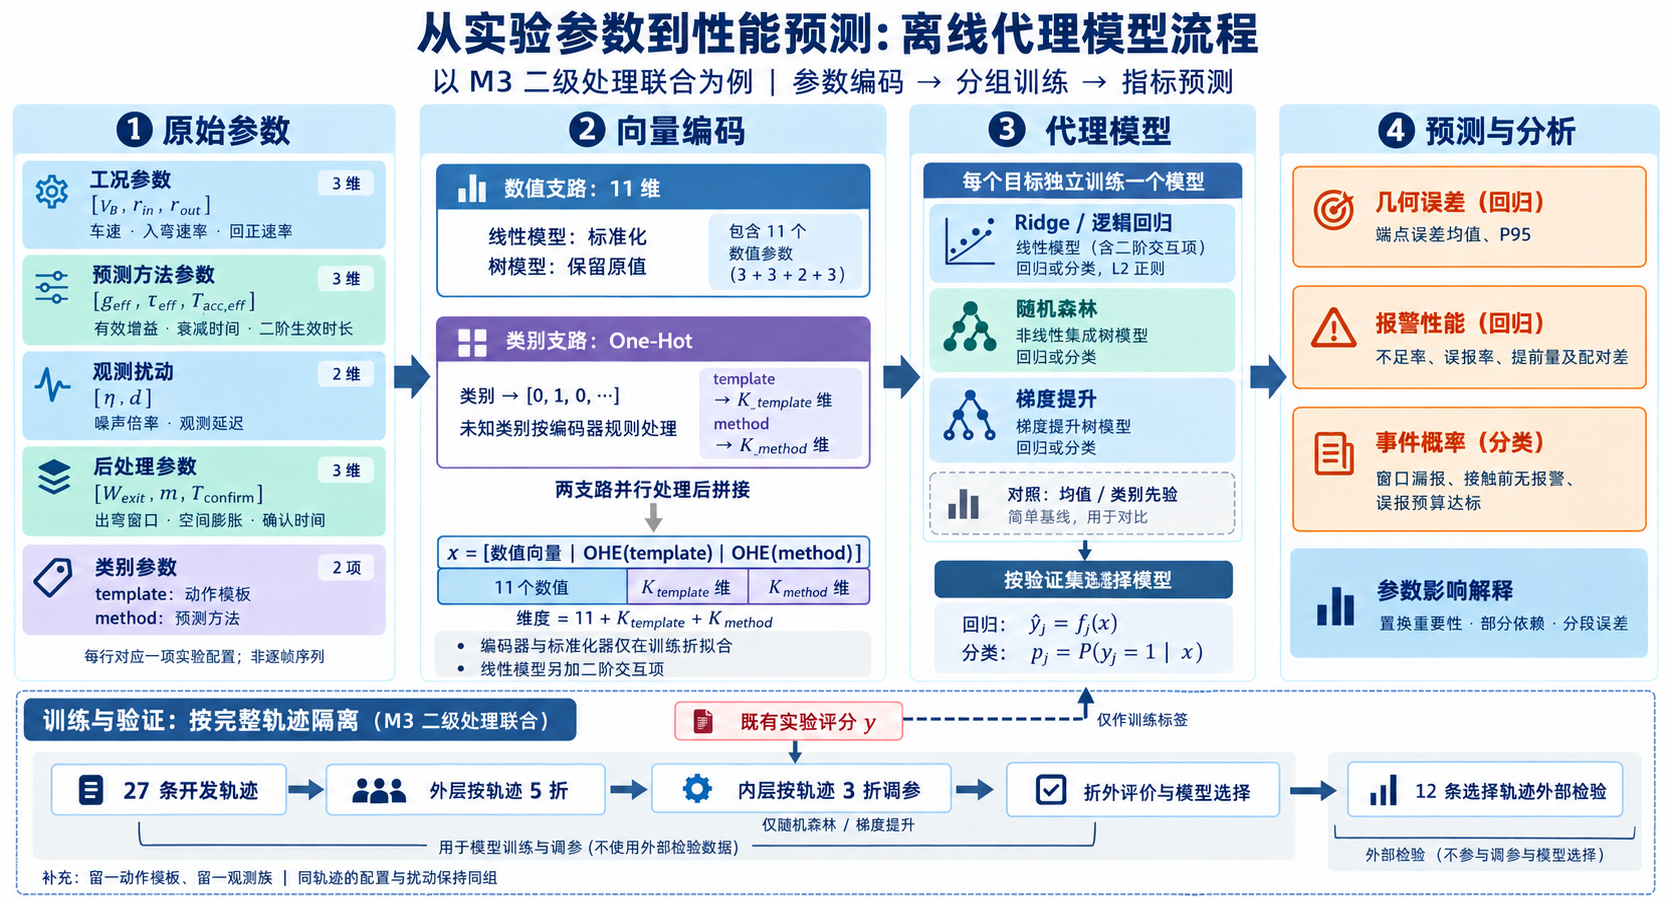
\includegraphics[width=0.93\textwidth,height=0.70\textheight,keepaspectratio]{img/arch_pipeline.png}
  \end{center}
  {\scriptsize\color{black!62}
  数值支路 11 维 = 工况 3 + 算法 3 + 观测 2 + 后处理 3；类别支路 = 动作模板 + 预测方法。
  方法专属参数按掩码处理：不适用时记 0。}
\end{frame}

\begin{frame}{B3\ \ 训练与验证：按完整轨迹隔离}
  \vspace{-0.4em}
  \begin{center}
    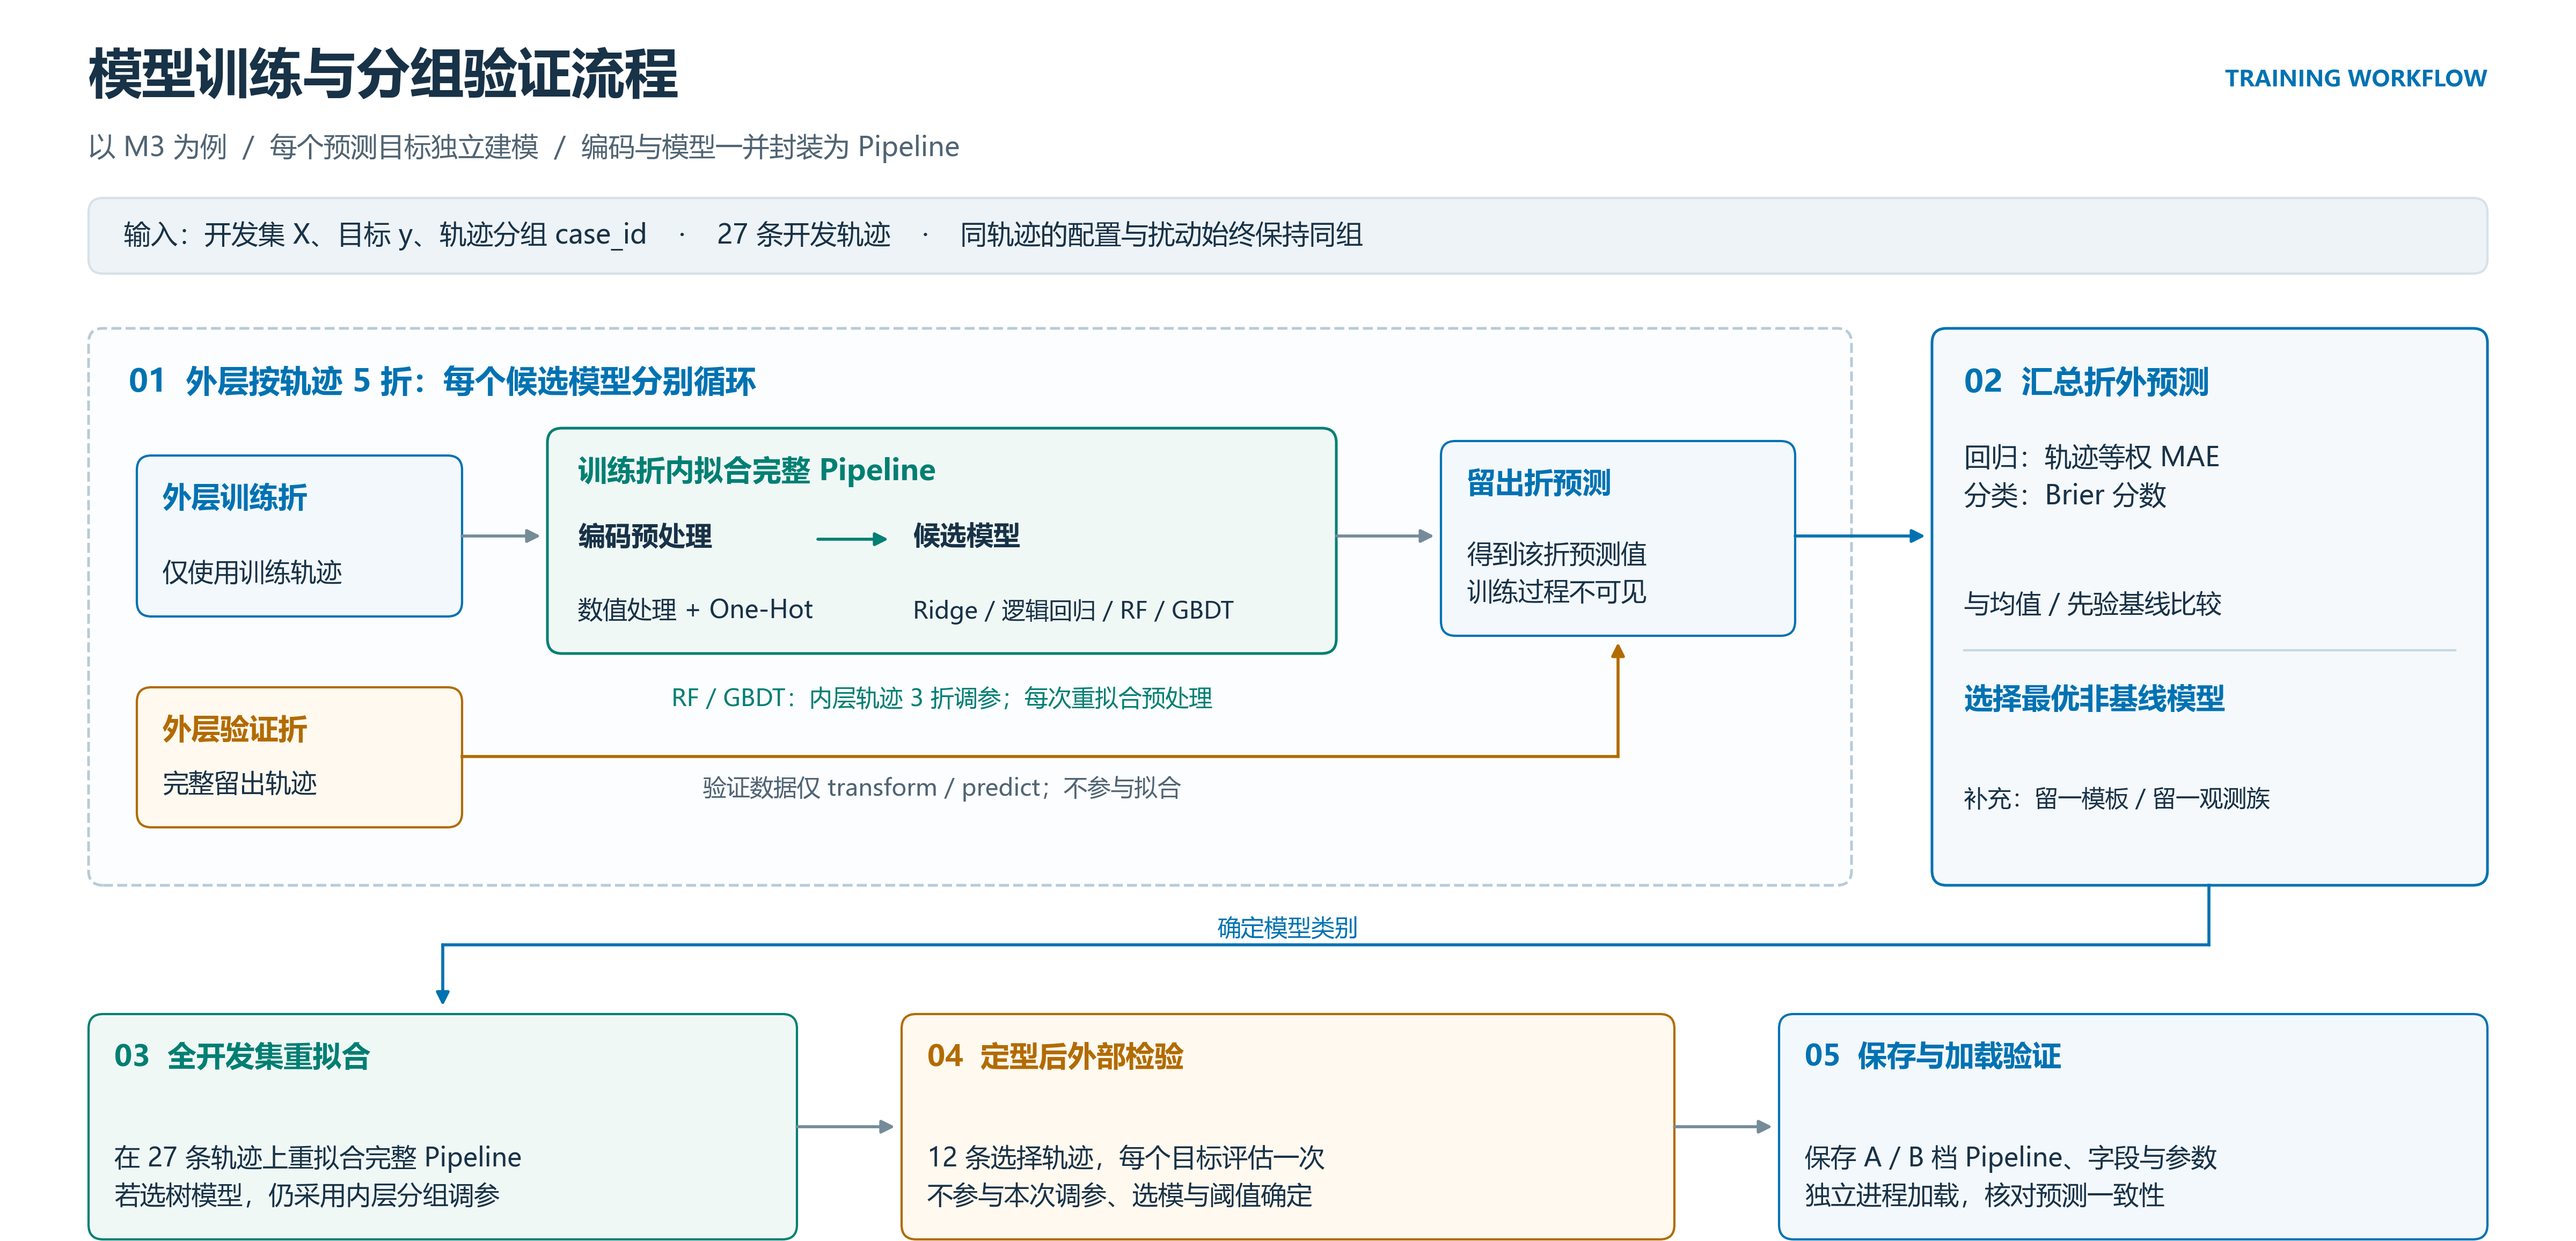
\includegraphics[width=0.95\textwidth,height=0.74\textheight,keepaspectratio]{img/arch_training.png}
  \end{center}
  {\scriptsize\color{black!62}
  \textbf{外层按轨迹 5 折}：同一条轨迹的所有行要么全在训练折、要么全在测试折，
  模型永远在\textbf{没见过的轨迹}上被评估。编码与标准化只在训练折内拟合。
  另设\textbf{留一动作模板}（每次留出 9 条同模板轨迹）作泛化诊断。}
\end{frame}

\begin{frame}{B4\ \ 五个模型族与数据}
  \centering
  \scriptsize
  \setlength{\tabcolsep}{3pt}\renewcommand{\arraystretch}{1.40}
  \begin{tabular}{@{}llcccl@{}}
    \toprule
    \textbf{模型族} & \textbf{数据} & \textbf{任务数} & \textbf{主验证} & \textbf{额外验证} & \textbf{回答什么} \\
    \midrule
    \textbf{M1} 核心方法 & D1：27 轨迹 / 513 行 & 9 & 按轨迹 5 折 & 留一模板 & 哪种 $\alpha$ 假设好 \\
    \textbf{M2a} 观测扰动 & D2：6 轨迹 / 864 行 & 7 & 留一轨迹 & — & 噪声延迟影响多大 \\
    \textbf{M2b} 状态估计 & D4：6 轨迹 / 576 行 & 10 & 留一轨迹 & — & EKF 能否补救 \\
    \textbf{M3} 后处理联合 & D3：39 轨迹 / 7{,}800 行 & 19 & 按轨迹 5 折 & 留一模板 + \textbf{外部} & 后处理怎么配 \\
    \textbf{M4} 增益精化 & D5：12 选择轨迹 / 8{,}064 行 & 19 & 按轨迹 4 折 & 留一模板 & 增益还有多少空间 \\
    \midrule
    \multicolumn{2}{@{}l}{\textbf{合计}} & \textbf{64} & \multicolumn{3}{l}{每个任务独立建模，分别预测漏报/迟报/误报/提前量/开销} \\
    \bottomrule
  \end{tabular}

  \vspace{0.6em}
  \begin{columns}[T]
    \begin{column}{0.49\textwidth}
      \footnotesize\textbf{候选模型（四类）}
      \begin{itemize}\tiny\setlength{\itemsep}{0pt}
        \item 基线：训练折均值 / 先验概率
        \item Ridge / 逻辑回归（含二阶交互）
        \item 随机森林
        \item 梯度提升
      \end{itemize}
    \end{column}
    \begin{column}{0.49\textwidth}
      \footnotesize\textbf{skill（相对基线的改善）}
      \[
      \text{skill}=1-\frac{\text{MAE}_{\text{模型}}}{\text{MAE}_{\text{基线}}}
      \]
      {\tiny MAE 先在每条轨迹内平均，再对轨迹等权平均。0 = 不比猜均值好，1 = 完全准确。}
    \end{column}
  \end{columns}
\end{frame}

\begin{frame}{B5\ \ M1：S1 的 9 个任务全部可学（A 档）}
  \vspace{-0.4em}
  \begin{columns}[T]
    \begin{column}{0.54\textwidth}
      \footnotesize
      \renewcommand{\arraystretch}{1.30}
      \begin{tabular}{@{}lc@{}}
        \toprule
        \textbf{预测目标} & \textbf{skill} \\
        \midrule
        0.3\,s 端点误差均值 & 0.86 \\
        2\,s 端点误差均值 & 0.79 \\
        2\,s 端点误差 P95 & 0.77 \\
        1\,s 端点误差均值 & 0.74 \\
        RIGHT 不足率 $-$ 保持 & 0.73 \\
        近场点误报率 $-$ 保持 & 0.72 \\
        RIGHT 不足率 & 0.70 \\
        近场点误报率 & 0.70 \\
        提前量 P10 $-$ 保持 & 0.57 \\
        \bottomrule
      \end{tabular}
      \vspace{0.4em}

      {\scriptsize\color{black!62}9 个任务全部达 A 档（skill $\ge$0.3 且 $R^2\ge$0.5）。}
    \end{column}
    \begin{column}{0.43\textwidth}
      \footnotesize
      \textbf{读法}\par
      每个任务单独建一个模型；skill 是相对「猜均值」基线的改善。

      \vspace{0.9em}
      \textbf{模型类别}\par
      最优模型 \textbf{8 个是梯度提升}，只有 2\,s 端点误差 P95 是 Ridge——
      尾部误差由少量极端值主导，线性模型反而更稳。

      \vspace{0.9em}
      \textbf{换一种分组方式}\par
      改用\textbf{留一动作模板}（每次整组留出同一模板的 9 条轨迹），
      多数任务 skill 不降反升，只有 P95 降到 \textbf{0.51}——
      尾部误差对没见过的动作模板更敏感。

      \vspace{0.9em}
      {\scriptsize\color{black!65}主方案的 skill 由同组外层成绩选出模型类别，略偏乐观。}
    \end{column}
  \end{columns}
\end{frame}

\begin{frame}{B6\ \ M1：折外预测紧贴对角线}
  \vspace{-0.45em}
  \begin{columns}[T]
    \begin{column}{0.50\textwidth}
      \begin{center}
      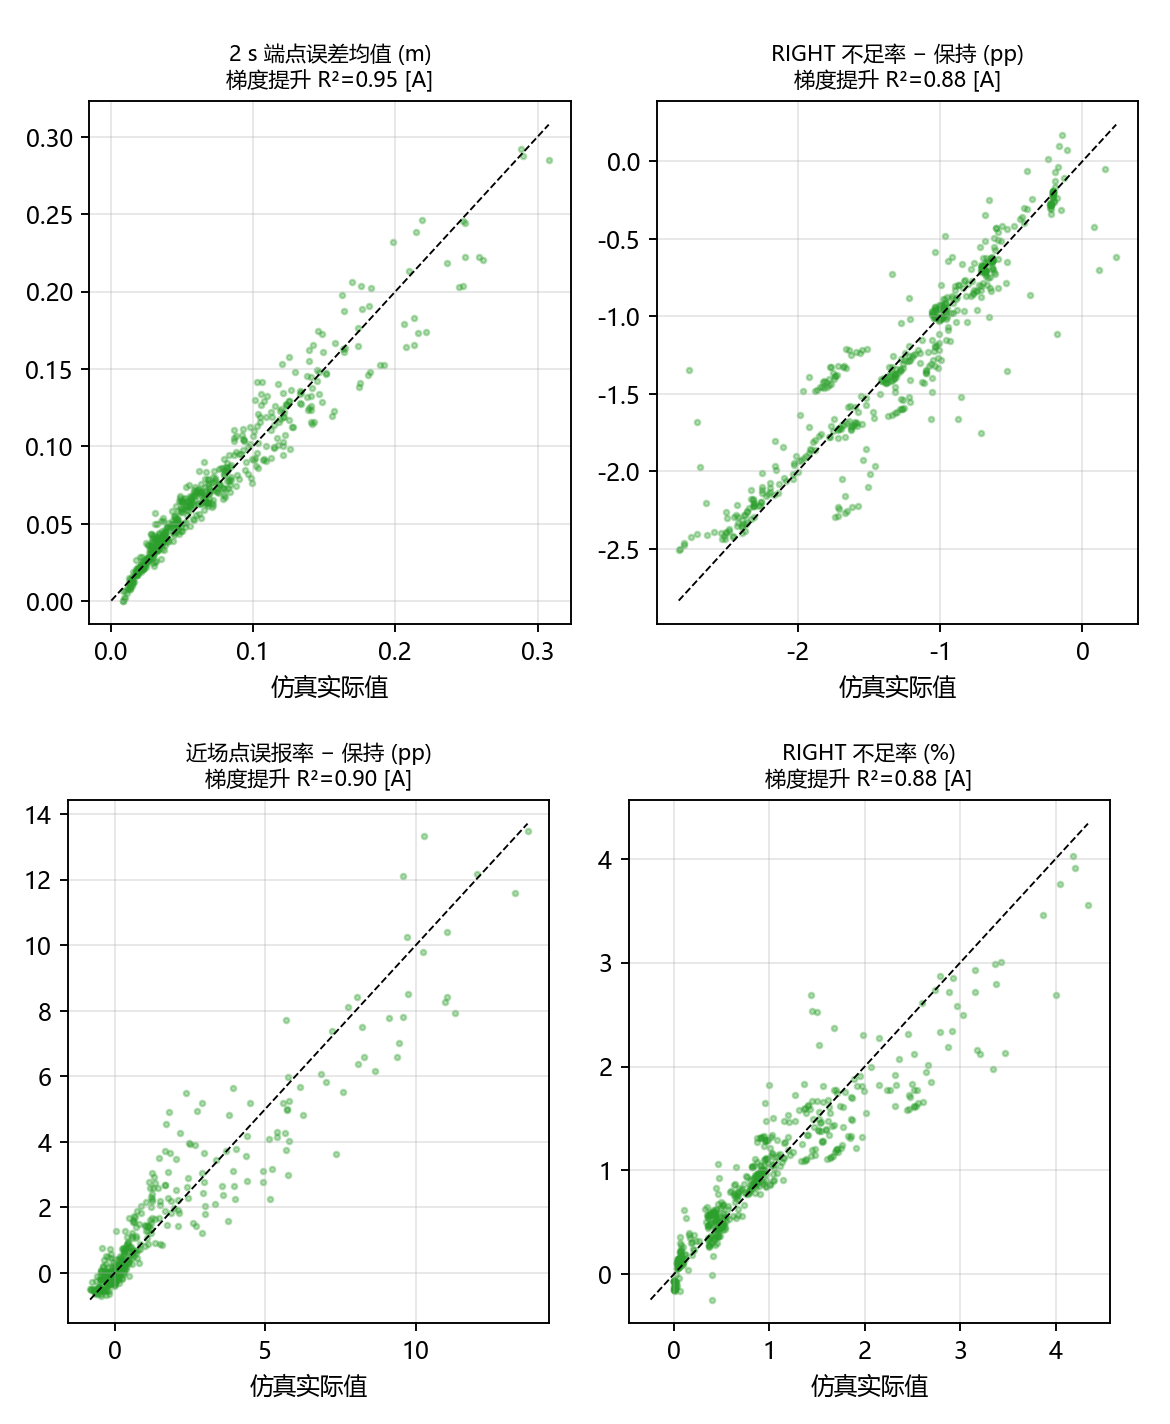
\includegraphics[width=\textwidth,height=0.735\textheight,keepaspectratio]{img/m1_f02_oof_2x2.png}
      \end{center}
    \end{column}
    \begin{column}{0.47\textwidth}
      \footnotesize
      \textbf{四个关键任务的 $R^2$}\par
      \vspace{0.3em}
      \renewcommand{\arraystretch}{1.3}
      \begin{tabular}{@{}lc@{}}
        \toprule
        预测目标 & $R^2$ \\
        \midrule
        2\,s 端点误差均值 & \textbf{0.945} \\
        RIGHT 不足率 $-$ 保持 & \textbf{0.879} \\
        近场误报率 $-$ 保持 & \textbf{0.899} \\
        RIGHT 不足率 & \textbf{0.877} \\
        \bottomrule
      \end{tabular}

      \vspace{0.9em}
      \textbf{怎么读}\par
      每个点 = 一条轨迹 × 一个配置，全部来自\textbf{训练时没见过的轨迹}（按轨迹 5 折的折外预测）。
      点越贴近虚线对角线越好。

      \vspace{0.6em}
      偏离最大的点来自 $v$=4\,m/s、$r$=8\,°/s 这类\textbf{最快最急}的轨迹——
      外推最难，但也没有系统性地偏向一侧。
    \end{column}
  \end{columns}
\end{frame}

\begin{frame}{B7\ \ M1：置换重要性}
  \vspace{-0.45em}
  \begin{columns}[T]
    \begin{column}{0.53\textwidth}
      \begin{center}
      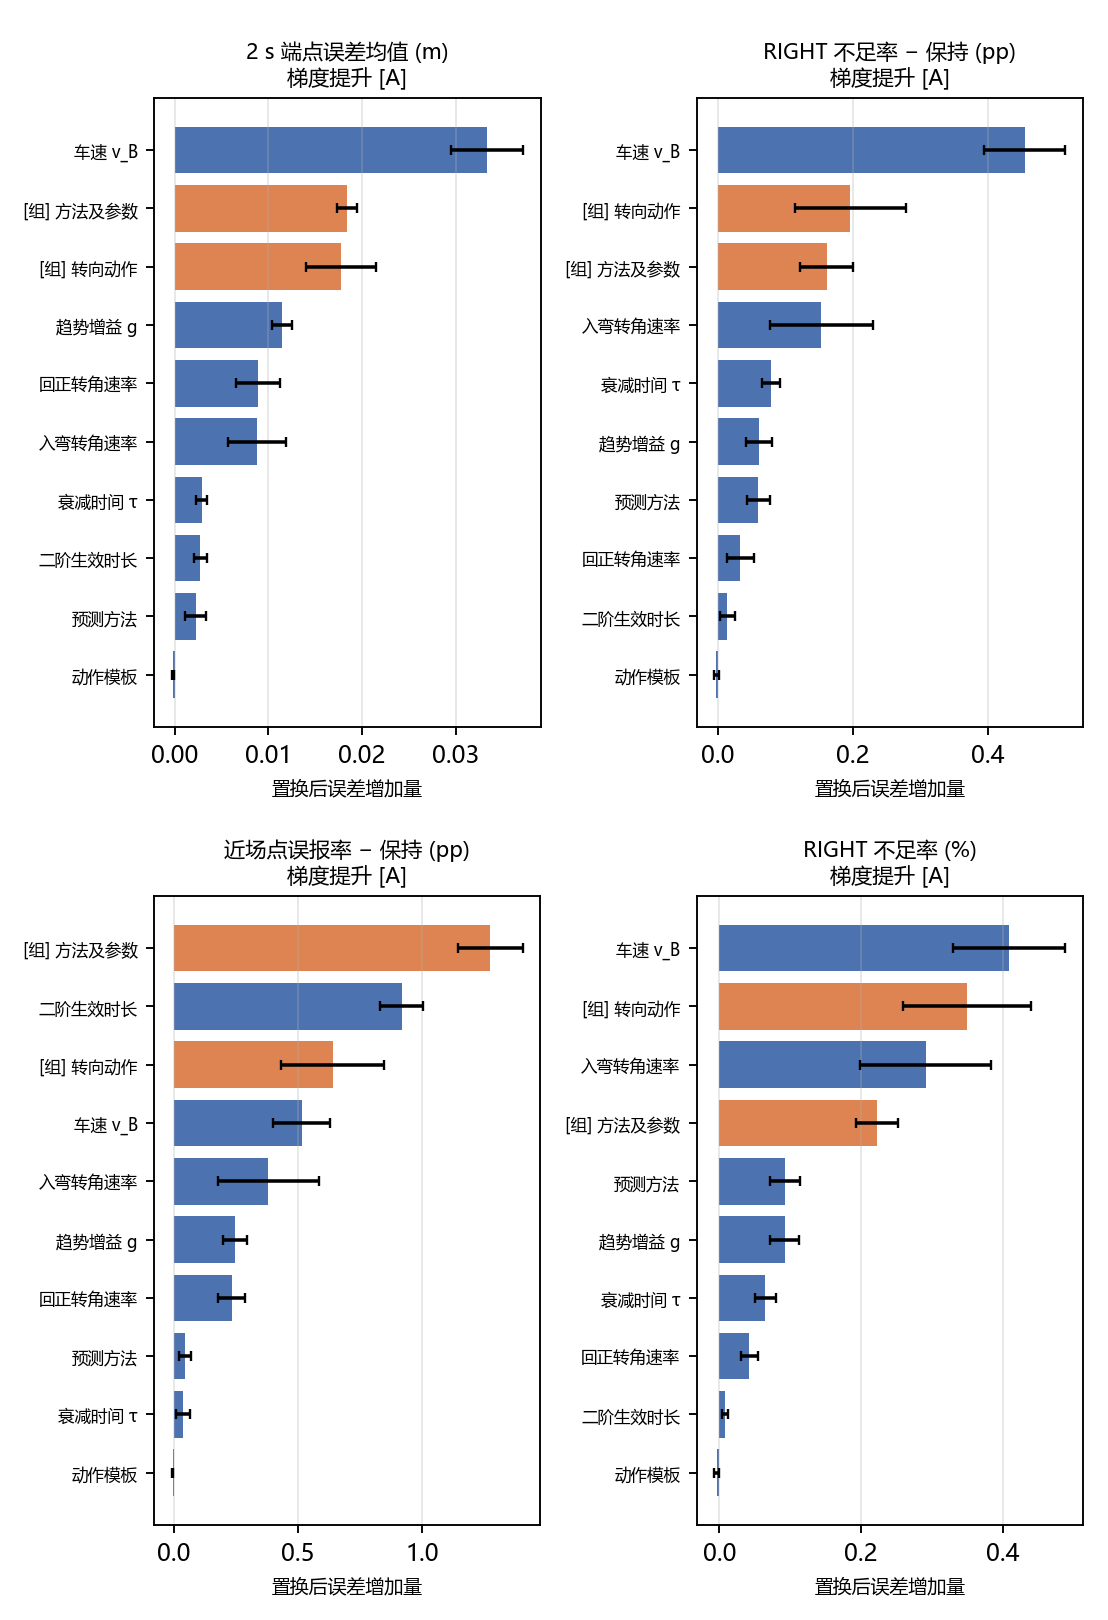
\includegraphics[width=\textwidth,height=0.735\textheight,keepaspectratio]{img/m1_f05_perm_2x2.png}
      \end{center}
    \end{column}
    \begin{column}{0.44\textwidth}
      \footnotesize
      \textbf{怎么读}\par
      打乱一个输入后折外误差增加多少；橙色是\textbf{成组置换}（一组相关输入一起打乱）。
      误差线为跨折标准差。

      \vspace{0.8em}
      \textbf{RIGHT 不足率 $-$ 保持}\par
      车速 \textbf{0.455} $>$ 转向动作组 0.197 $>$ 方法及参数组 0.161
      ——与「收益随车速与转向速率增大」一致。

      \vspace{0.7em}
      \textbf{近场误报率 $-$ 保持}\par
      方法及参数组 \textbf{1.28}，其中二阶生效时长 \textbf{0.918}——误报代价主要由参数决定。

      \vspace{0.7em}
      \textbf{2\,s 端点误差}\par
      车速 \textbf{0.033\,m} 最重要。

      \vspace{0.8em}
      {\scriptsize\color{black!65}重要性描述模型的依赖关系，\textbf{不等于因果}。}
    \end{column}
  \end{columns}
\end{frame}

\begin{frame}{B8\ \ M3（主模型）：19 个任务全部 A 档}
  \vspace{-0.5em}
  \begin{columns}[T]
    \begin{column}{0.47\textwidth}
      \scriptsize
      \renewcommand{\arraystretch}{1.14}
      \begin{tabular}{@{}lc@{}}
        \toprule
        \textbf{预测目标} & \textbf{skill} \\
        \midrule
        2\,s 端点误差均值 & 0.95 \\
        共同 2\,s 帧误报 $-$ 无后处理 & 0.95 \\
        共同 2\,s 帧误报 $-$ 保持 & 0.95 \\
        共同 2\,s 逐帧误报率 & 0.93 \\
        逐帧误报率 & 0.93 \\
        近场误报 $-$ 无后处理 & 0.92 \\
        近场点误报率 & 0.91 \\
        提前量 P10 & 0.90 \\
        近场误报 $-$ 保持 & 0.90 \\
        误报预算达标 & 0.90 \\
        接触前完全无报警 & 0.82 \\
        出现窗口漏报 & 0.82 \\
        RIGHT 不足率 $-$ 无后处理 & 0.81 \\
        提前量 P10 $-$ 保持 & 0.81 \\
        2\,s 端点误差 P95 & 0.79 \\
        RIGHT 不足率 & 0.78 \\
        窗口漏报率 & 0.74 \\
        窗口漏报 $-$ 无后处理 & 0.74 \\
        RIGHT 不足率 $-$ 保持 & 0.72 \\
        \bottomrule
      \end{tabular}
      \vspace{0.4em}

      {\scriptsize\color{black!62}19 个 $=$ 16 回归 $+$ 3 分类，全部 A 档。}
    \end{column}
    \begin{column}{0.50\textwidth}
      \footnotesize
      \textbf{M3 是什么}\par
      把\textbf{后处理三参数}（出弯窗口、膨胀、确认时间）作为输入的模型族，
      用 27 条开发轨迹的 \textbf{5{,}400 行}训练。这是本项目的\textbf{主模型族}。

      \vspace{1.0em}
      \textbf{分工}\par
      M1 只回答「哪种 $\alpha(u)$ 假设好」；
      M3 回答「后处理该怎么配」——后者才是工程上能调的旋钮。

      \vspace{1.0em}
      \textbf{最难的三个}\par
      RIGHT 不足率 $-$ 保持（0.72）、窗口漏报率（0.74）及相对无后处理的变化（0.74）：
      都涉及「有没有漏掉」这类离散事件，比连续量难学。

      \vspace{1.0em}
      {\scriptsize\color{black!65}外部检验见下一页。}
    \end{column}
  \end{columns}
\end{frame}

\begin{frame}{B9\ \ M3：外部检验——规律能推广到新轨迹}
  \vspace{-0.45em}
  \begin{columns}[T]
    \begin{column}{0.50\textwidth}
      \begin{center}
      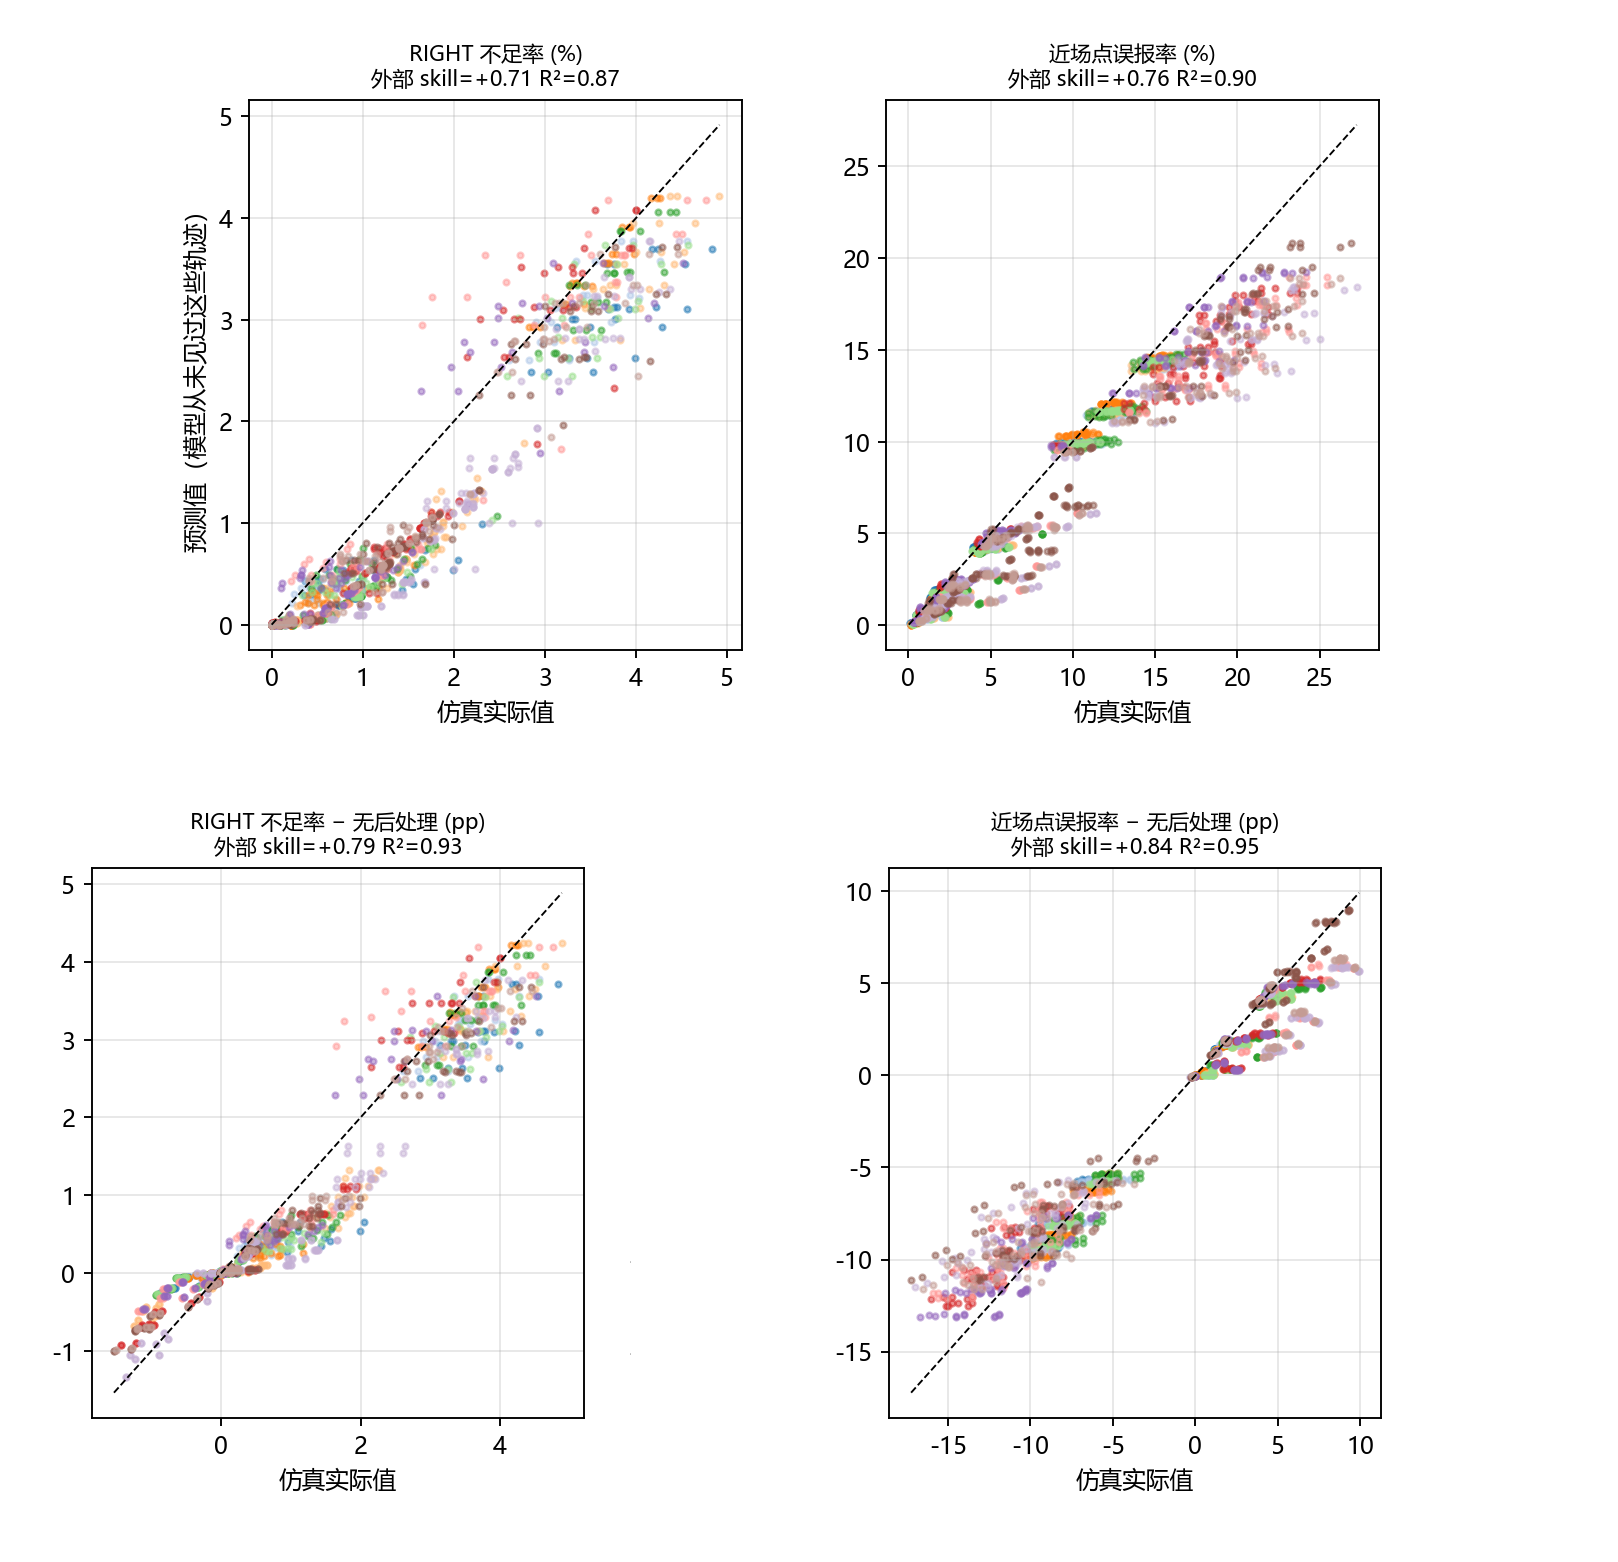
\includegraphics[width=\textwidth,height=0.70\textheight,keepaspectratio]{img/m3_f08_external_2x2.png}
      \end{center}
    \end{column}
    \begin{column}{0.47\textwidth}
      \footnotesize
      \textbf{四个目标的外部 skill / $R^2$}\par
      \vspace{0.3em}
      \renewcommand{\arraystretch}{1.3}
      \begin{tabular}{@{}lcc@{}}
        \toprule
        预测目标 & skill & $R^2$ \\
        \midrule
        RIGHT 不足率 & 0.71 & 0.87 \\
        近场误报率 & 0.76 & 0.90 \\
        RIGHT 不足率 $-$ 无后处理 & 0.79 & 0.93 \\
        近场误报率 $-$ 无后处理 & 0.84 & 0.95 \\
        \bottomrule
      \end{tabular}

      \vspace{0.9em}
      \textbf{为什么这条证据最硬}\par
      12 条选择轨迹\textbf{不参与训练、调参、阈值选择和学习曲线}，每个目标只评估一次。

      \vspace{0.7em}
      \textbf{代价}\par
      外部 skill 普遍低于主方案（主方案 0.71--0.95 vs 外部 0.71--0.84），
      说明主方案成绩中的「最优模型类别」是在同一组外层成绩上选的，\textbf{略偏乐观}。
      未列入表的 2\,s 端点误差均值外部 skill 最低（0.48）——几何误差在轨迹间波动最大。
    \end{column}
  \end{columns}
\end{frame}

\begin{frame}{B10\ \ M3：后处理参数的部分依赖}
  \vspace{-0.55em}
  \begin{center}
  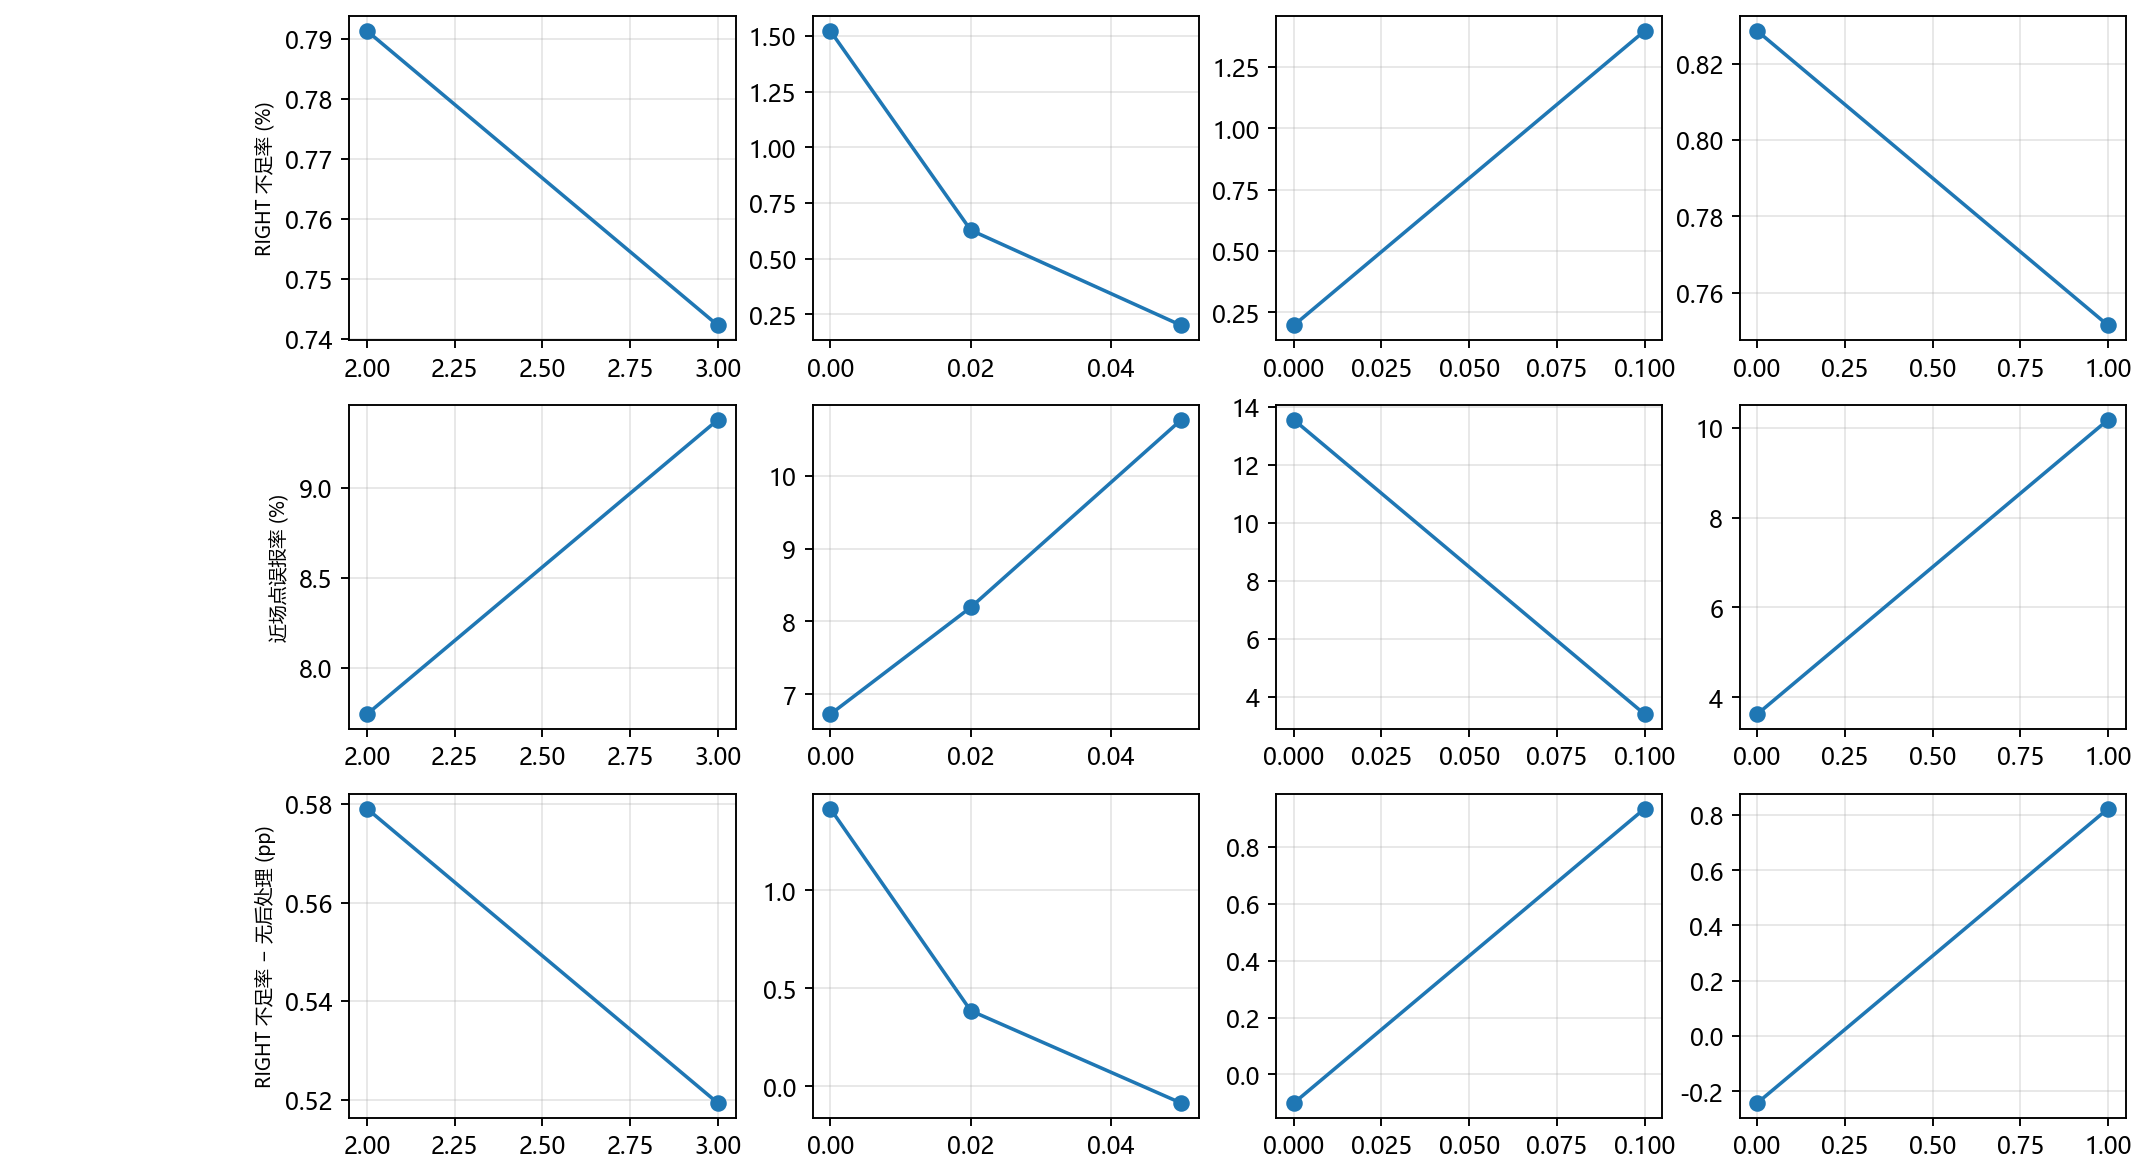
\includegraphics[width=0.80\textwidth,height=0.655\textheight,keepaspectratio]{img/m3_f10_pdp_crop.png}
  \end{center}
  \vspace{-0.9em}
  {\scriptsize\color{black!62}%
  \textbf{列}=出弯窗口 $W$/膨胀/确认时间/噪声倍率；\textbf{行}=RIGHT 不足率、近场点误报率、相对无后处理的迟报变化。\par}
  \vspace{0.35em}
  {\footnotesize
  三行方向互相矛盾，正是 S3 的结论：确认时间压误报但抬高迟报，膨胀相反；出弯窗口 2→3\,s 只抬误报。
  代理模型独立复现了 S3 的配对效应方向。}
\end{frame}

\begin{frame}{B11\ \ 全部 64 个任务的临时表现分档}
  \vspace{-0.45em}
  \begin{center}
  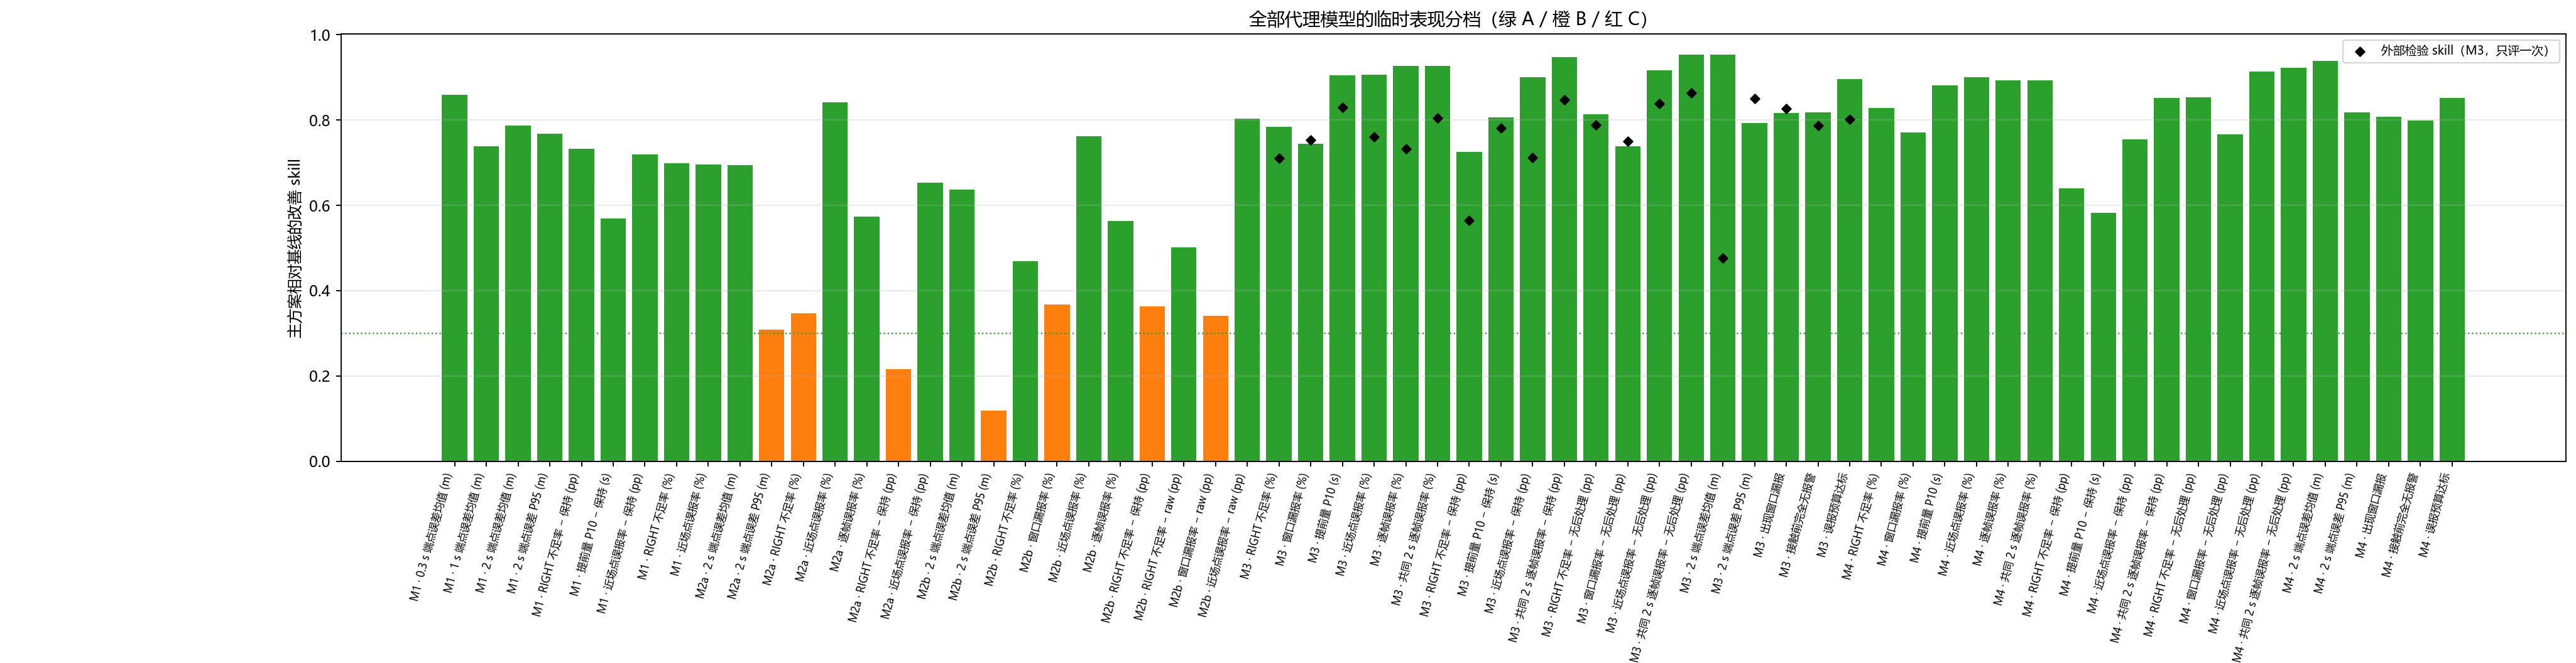
\includegraphics[width=0.97\textwidth,height=0.585\textheight,keepaspectratio]{img/all_f11_tiers.png}
  \end{center}
  \vspace{-0.55em}
  {\scriptsize\color{black!62}每根柱 = 一个「模型族 × 预测目标」任务的主方案 skill（折外）；绿 A / 橙 B / 红 C。\par}
  \vspace{0.5em}
  {\footnotesize
  \textbf{A 档 57 个、B 档 7 个、C 档 0 个}。B 档全部落在 M2a/M2b——这两族只有 6 条轨迹，组数不足限制了解释力。
  \textbf{分档口径}：A 档 $=$ 主方案 skill $\ge$0.3 且 $R^2\ge$0.5（分类 AUC $\ge$0.75）、所有验证方案优于基线；B 档 $=$ 优于基线但未达 A。
  分档只衡量\textbf{对已有评分的预测能力}，不是科研准入。}
\end{frame}

\begin{frame}{B12\ \ 这一部分想说明什么}
  \begin{columns}[T]
    \begin{column}{0.48\textwidth}
      \begin{block}{已经说明的}
        \footnotesize
        \begin{itemize}\setlength{\itemsep}{2pt}
          \item S1 的 9 个任务全部可学，换动作模板仍成立
          \item M3 在 12 条未见轨迹上外部 skill 0.48--0.86
          \item 车速是迟报收益的首要因素
          \item 初始二阶的生效时长是误报代价的首要因素
          \item 代理模型复现了 S3 的配对效应方向
        \end{itemize}
      \end{block}
    \end{column}
    \begin{column}{0.48\textwidth}
      \begin{alertblock}{尚未说明的}
        \footnotesize
        \begin{itemize}\setlength{\itemsep}{2pt}
          \item 只覆盖\textbf{一种转弯几何}（10° 转角、22.7\,m 半径）
          \item 选择集外部检验是\textbf{同几何内部的内插}，不是真正的外推
          \item M2a/M2b 只有 6 条轨迹，稳健性有限
          \item 绝对值指标只作描述，不作部署依据
          \item 没有实车数据，也没有 MCU 计时
        \end{itemize}
      \end{alertblock}
    \end{column}
  \end{columns}

  \vspace{0.5em}
  \begin{block}{一句话}
    \small 代理模型证明的是「\textbf{规律稳定且可学}」，不是「\textbf{参数已最优}」。
  \end{block}
\end{frame}

\end{document}
